% !TeX program = xelatex
% build_report.py fills the data placeholders; report.tex is standalone.
\documentclass[11pt,a4paper]{article}
\usepackage{kotex}
\IfFontExistsTF{UnBatang.ttf}{
 \setmainhangulfont{UnBatang.ttf}[BoldFont=UnBatangBold.ttf,
  ItalicFont=UnBatang.ttf,BoldItalicFont=UnBatangBold.ttf,
  Script=Hangul,Language=Korean]
}{}
\usepackage[margin=23mm,headheight=16pt]{geometry}
\usepackage{amsmath,amssymb,mathtools,bm}
\usepackage{booktabs,tabularx,array,longtable}
\usepackage[dvipsnames]{xcolor}
\usepackage{tikz,pgfplots}
\usetikzlibrary{arrows.meta,positioning,calc}
\usepgfplotslibrary{groupplots}
\pgfplotsset{compat=1.18}
\usepackage{enumitem,fancyhdr,xurl,float,needspace,listings}
\usepackage[unicode,colorlinks=true,linkcolor=MidnightBlue,
 citecolor=MidnightBlue,urlcolor=MidnightBlue,
 pdftitle={과제 내 시간 표현과 과제 간 상호작용을 이용한 PD/ET 분류 실험 보고서}]{hyperref}
\definecolor{navy}{HTML}{224C70}
\definecolor{orangeplot}{HTML}{D27A27}
\definecolor{redplot}{HTML}{B44446}
\definecolor{greenplot}{HTML}{3F8064}
\definecolor{purpleplot}{HTML}{8560A6}
\definecolor{softgray}{HTML}{F4F6F8}
\newcommand{\R}{\mathbb{R}}
\newcommand{\ind}{\mathbf{1}}
\newcommand{\code}[1]{\texttt{\detokenize{#1}}}
\DeclareMathOperator{\BA}{BA}
\DeclareMathOperator{\mean}{mean}
\DeclareMathOperator{\sd}{sd}
\DeclareMathOperator{\GELU}{GELU}
\DeclareMathOperator{\LN}{LayerNorm}
\DeclareMathOperator{\concat}{concat}
\setlength{\parindent}{0pt}
\setlength{\parskip}{0.42em}
\setlength{\emergencystretch}{2.5em}
\renewcommand{\arraystretch}{1.17}
\clubpenalty=10000 \widowpenalty=10000
\numberwithin{equation}{section}
\setlist[itemize]{leftmargin=1.5em,itemsep=.2em,topsep=.3em}
\setlist[enumerate]{leftmargin=1.8em,itemsep=.25em,topsep=.3em}
\renewcommand{\abstractname}{초록}
\renewcommand{\contentsname}{목차}
\renewcommand{\figurename}{그림}
\renewcommand{\tablename}{표}
\renewcommand{\refname}{참고문헌}
\setcounter{tocdepth}{1}
\pagestyle{fancy}\fancyhf{}
\fancyhead[L]{\small\color{navy}PADS PD/ET: 시간 표현 및 과제 간 결합}
\fancyhead[R]{\small 실험 결과 보고서}
\fancyfoot[C]{\thepage}
\renewcommand{\headrulewidth}{.3pt}
\lstset{basicstyle=\ttfamily\footnotesize,backgroundcolor=\color{softgray},
 frame=single,rulecolor=\color{gray!25},breaklines=true,columns=fullflexible,
 keepspaces=true,showstringspaces=false}
\newenvironment{keybox}{\begin{center}\begin{minipage}{.94\linewidth}\color{navy}\hrule\vspace{.6em}\small}
 {\vspace{.5em}\hrule\end{minipage}\end{center}}

\title{\color{navy}\bfseries 과제 내 시간 표현과 과제 간 상호작용을\\[.25em]
 결합한 PD/ET 분류 실험 보고서\\[.6em]
 \large PADS 참가자 단위 5\,$\times$\,3 중첩 교차검증과 구성요소 제거 분석}
\author{PD/ET Classification Project}
\date{2026년 11월 8일\\[.25em]\small 완료 실행: \code{20261108T071720522119Z}}

\begin{document}
\maketitle\thispagestyle{empty}
\begin{abstract}
PADS v1.0.0의 파킨슨병(PD) 276명과 본태성 떨림(ET) 28명을 대상으로,
과제 내 시간 표현과 과제 간 저랭크 상호작용을 결합한 경량 신경망을 평가하였다.
안정 시, 인지 부하 안정 시, 자세 조건의 양측 손목 가속도 및 각속도에서
동일한 60채널 입력을 구성하였다. 공유 윈도 CNN, 작은 Transformer,
쌍선형 과제 결합으로 이루어진 전체 모델과 네 가지 신경망 대조군,
Frozen MantisV2 및 MultiROCKET--HYDRA를 같은 참가자 분할로 비교하였다.
외부 5-fold, 내부 3-fold, 1회 반복의 중첩 교차검증에서 전체 모델의
균형 정확도는 56.16\%, ET 민감도는 25.00\%(7/28), PD 특이도는 87.32\%였다.
두 모듈을 모두 제거한 모델은 균형 정확도 61.57\%, MantisV2는 61.05\%였으며,
MultiROCKET--HYDRA는 pooled AUROC 0.8612로 가장 높은 순위 구별력을 보였다.
전체 모델과 각 대조군의 BA 차이에 대한 조건부 대응 bootstrap 구간은 모두 0을 포함하였다.
따라서 \textbf{이번 실행은 제안 구조의 성능 향상 가설을 지지하지 않는다.}
이 결론은 특정 구현과 탐색 범위에 한정되며, 해당 개념 전체의 무용성을 뜻하지 않는다.
보고서의 모든 평가 지표는 저장된 외부 예측에서 다시 계산하였고,
새로운 학습이나 모델 예측은 수행하지 않았다.
\end{abstract}

\begin{keybox}
\textbf{읽을 때의 기준.}
독립 분석 단위는 참가자 한 명이다. 양성은 ET($y=1$), 음성은 PD($y=0$)다.
주 성능은 참가자별 외부 평가 예측을 합친 BA이다.
내부 선택 점수, 학습 손실, 전체 304명으로 적합한 최종 모델의 학습 자료 성능은
독립 평가 성능이 아니다. 출력 점수는 보정된 임상 확률이 아니다.
\end{keybox}
\clearpage
\tableofcontents
\vfill
\begin{keybox}
\textbf{보고서 구성.}
실행 자료와 모델의 정의를 먼저 제시한 뒤, 검증 절차, 전체 비교,
구성요소 제거 분석과 불확실성을 설명한다. 부록에는 35개 외부 평가 fold의
선택 설정과 결과, 과거 132채널 결과와의 구분, 감사 및 재현 정보를 수록한다.
\end{keybox}
\clearpage

\section{연구 질문과 분석 범위}

본 연구의 질문은 같은 참가자에게서 얻은 서로 다른 과제 조건의 신호를
구조적으로 결합하면 PD와 ET를 더 잘 구별할 수 있는가이다.
여기서 시간적 변화는 수초에서 수십 초의 \textbf{과제 기록 내 변화}를 뜻한다.
장기간의 질병 진행이나 치료 전후 변화를 추정하는 종단 연구가 아니다.
과제 간 상호작용은 다른 조건의 특징들이 함께 나타날 때 분류 점수에 미치는
효과를 학습하는 것으로 정의하며, 신경생리학적 인과 상호작용과 구분한다.

연구 가설은 다음 세 가지로 나눈다.
\begin{enumerate}
 \item 같은 국소 윈도 특징을 사용하더라도 과제 내 윈도 순서를 처리하는
 시간 인코더가 순서 없는 요약보다 유용한가.
 \item 과제별 점수의 합에 명시적인 과제 간 곱항을 추가하면 유용한가.
 \item 두 모듈을 결합한 전체 모델이 동일 입력의 기존 기준선보다 나은가.
\end{enumerate}
이 질문을 위해 일곱 방법을 각각 내부 검증으로 조정한 뒤 외부 참가자에서
평가하였다. 과거에 같은 코호트의 결과를 확인한 뒤 설계한 후속 실험이므로,
중첩 교차검증을 사용하더라도 본 분석은 \textbf{탐색적 연구}로 해석한다.
일곱 방법 중 외부 BA가 가장 높은 방법을 사후 선택해 새로운 최종 선택 절차의
성능으로 주장하지 않는다.

주파수의 시간적 변동을 감별에 쓰는 발상은 이미 Tremor Stability Index 연구에
있으며\cite{tsi}, 여러 자세와 센서 신호를 CNN 및 attention으로 결합한 연구도
존재한다\cite{mfca}. PADS 양측 손목 attention과 새로운 과제로의 일반화를
분석한 사전공개 연구\cite{bilateral}도 있으나, 주로 PD/건강인 및 PD/여러
감별진단을 다루므로 현재 PD/ET 이진 문제와 성능을 직접 비교하지 않는다.
따라서 특정 구현의 효용과 독창성은 구분해야 한다. 본 실험은 구성요소 자체의
최초 발명이나 기존 시계열 모델이 시간 정보를 학습하지 못한다는 주장을 하지 않는다.

\section{데이터, 입력 표현과 시간축}
\subsection{참가자와 정답 정의}
자료는 PADS v1.0.0\cite{pads,padsstudy}다. 참가자 $i\in\{1,\ldots,N\}$,
$N=304$에 대해 공식 진단 문자열이 \code{Parkinson's}이면 $y_i=0$,
\code{Essential Tremor}이면 $y_i=1$로 정한다. PD는 276명, ET는 28명이다.
원래 숫자 라벨 2에는 ET 외의 감별진단도 포함되어 있어 이를 ET로 간주하지 않는다.
PD로 배정되었지만 설명에 ET가 언급된 8명도 공식 라벨을 유지한다.
진단 설명, 인구학적 변수, 설문, 약물 정보와 참가자 ID는 입력 특징에 포함하지 않는다.

\subsection{세 조건과 다섯 구간}
\begin{table}[H]\centering\small
\caption{분석에 사용한 조건과 공식 전처리 구간. 각 구간은 12채널\,$\times$\,976샘플이다.}
\begin{tabularx}{\linewidth}{@{}lXl@{}}\toprule
 조건 $q$ & 공식 구간 이름 & 윈도 수 $K_q$\\\midrule
 안정 시 $r$ & \code{Relaxed1}, \code{Relaxed2} & 8\\
 인지 부하 안정 시 $c$ & \code{RelaxedTask1}, \code{RelaxedTask2} & 8\\
 자세 조건 $p$ & \code{StretchHold} & 4\\\bottomrule
\end{tabularx}\label{tab:inputs}
\end{table}
인지 조건은 안정 자세에서 연속 7 빼기를 수행한 조건이다\cite{pads}.
안정 자세와 인지 과제를 서로 배타적인 운동 상태로 취급하지 않는다.
자세 조건은 이 실행에서 \code{StretchHold}로 정하였으며,
다른 자세 기록이나 무게 들기 과제를 추가하지 않았다.

각 구간의 12채널은 왼쪽 손목 가속도 XYZ, 왼쪽 손목 각속도 XYZ,
오른쪽 손목 가속도 XYZ, 오른쪽 손목 각속도 XYZ 순서다.
원자료의 가속도 단위는 g, 각속도 단위는 rad/s, 명목 샘플링률은 100 Hz다.
공식 전처리는 중력 성분 추정 제거, 구간 선택과 앞부분 자르기를 포함한다.
새로운 임의 대역통과 필터나 과제별 자기 표준편차 정규화는 추가하지 않았다.

기존 공식 바이너리 $(132,976)$에서 앞의 다섯 구간에 해당하는 60채널을 선택한다.
신경망은 $X_i\in\R^{5\times12\times976}$를 받고,
두 기준선은 \textbf{동일한 값}을 재배열한 $\R^{60\times976}$ 입력을 받는다.
60채널이 모두 같은 시각에 기록된 물리 축이라는 뜻은 아니다.
다른 과제의 같은 샘플 번호를 같은 생리 사건으로 정렬하지 않는다.

\subsection{윈도와 잘린 구간 경계}
각 길이 976 구간을 길이 $L=244$인 네 윈도로 나눈다. 명목상 한 윈도는
2.44초다. 윈도 CNN은 각각을 따로 처리하므로 과제나 구간 경계를 가로질러
합성곱하지 않는다. 두 반쪽을 아무 표시 없이 한 파형으로 연결하지 않는다.

공식 로더는 긴 기록을 1,024샘플씩 나눈 뒤 각 구간 앞 48샘플을 제거하였다.
반쪽 번호 $h\in\{0,1\}$, 반쪽 내부 윈도 $j\in\{0,1,2,3\}$의 명목 위치는
\begin{equation}
 \tau_{hj}=\frac{48+(j+1/2)244+1024h}{100}\quad\text{(명목 초)}
\end{equation}
로 부여한다. 자세 조건에는 $h=0$만 있다. 위치 정보는 이 명목 시간에 대한
sin/cos 부호화다. \textbf{실제 원자료 타임스탬프는 복원하지 않았다.}
따라서 원자료의 비균일 샘플링이나 긴 시간 간격은 해결되지 않으며,
이 위치 정보가 실제 시계 시간과 정확히 같다고 해석할 수 없다.

\section{전체 모델의 수학적 구조}
\subsection{학습 집합에만 적합하는 공유 표준화}
하나의 적합에 사용한 참가자 집합을 $\mathcal I$, 그 크기를 $n$이라 하자.
물리 채널 $a\in\{1,\ldots,12\}$별로 $\mathcal I$의 모든 선택 구간과 샘플에서
평균 $\mu_a$와 모집단 표준편차 $\sigma_a$를 구한다. $\sigma_a$는 최소
$10^{-6}$으로 제한한다. 입력은
\begin{equation}
 \widetilde X_{i,s,a,t}=\frac{X_{i,s,a,t}-\mu_a}{\sigma_a},
 \qquad s\in\{1,\ldots,5\},\ t\in\{0,\ldots,975\}
\end{equation}
로 변환한다. 같은 12개 통계를 모든 과제와 검증/평가 참가자에게 적용한다.
각 참가자ㆍ과제를 자기 표준편차로 나누지 않으므로 과제 간 진폭 차이를
그 방식으로 제거하지 않는다. 다만 변환 후 진폭은 원래 물리 단위의 진폭이 아니다.

\subsection{공유 윈도 CNN과 진폭 특징}
표준화된 입력에서 분리한 윈도 $W_{i,q,k}\in\R^{12\times244}$에서 채널별 log-RMS를
\begin{equation}
 A_{i,q,k,a}=\log\sqrt{\frac1{244}\sum_{t=0}^{243}W_{i,q,k,a,t}^{\,2}+10^{-8}}
 \label{eq:rms}
\end{equation}
로 계산한다. CNN의 채널 수는 $12\to32\to32\to32$, 커널 크기는
7, 5, 3이며 stride는 모두 2다. 각 합성곱 뒤에 GELU를 적용한다.
padding을 포함한 시간 길이는 $244\to122\to61\to31$이다.
합성곱 출력 $F_{i,q,k}\in\R^{32\times31}$의 시간 평균과 최댓값,
$A_{i,q,k}\in\R^{12}$를 결합한 76차원 벡터를 만든다.
\begin{equation}
 u_{i,q,k}=\operatorname{Dropout}\!\left[\GELU\!\left(\LN\!\left(
 P\begin{bmatrix}\mean_t F_{i,q,k}\\\max_t F_{i,q,k}\\ A_{i,q,k}\end{bmatrix}+b_P
 \right)\right)\right]\in\R^{32},
\end{equation}
여기서 $P\in\R^{32\times76}$, $b_P\in\R^{32}$는 학습 모수다.
같은 CNN과 투영을 모든 윈도ㆍ과제에 사용한다.

\subsection{과제 내 순서 인코더와 요약}
과제 $q\in\{r,c,p\}$의 $K_q$개 특징에 명목 위치 정보를 더한 뒤,
과제 사이에 가중치를 공유하는 1-layer, 4-head Transformer를 적용한다.
은닉 차원은 32, feed-forward 차원은 64, dropout은 0.2다.
pre-norm 구성이며 활성화는 GELU다. 이 단계에서는 다른 과제의 토큰을 섞지 않는다.
출력 토큰을 $H_{i,q,k}\in\R^{32}$라 할 때
\begin{equation}
 z_i^q=\concat\!\left(
 \mean_k H_{i,q,k},\ \sd_k H_{i,q,k},\
 \mean_k A_{i,q,k},\ \sd_k A_{i,q,k}\right)\in\R^{88}
 \label{eq:taskfeature}
\end{equation}
로 요약한다. 표준편차는 분모 $K_q$를 쓰는 모집단 표준편차다.
차원은 $32+32+12+12=88$이다. 순서 인코더를 제거한 대조군에서는
$H_{i,q,k}=u_{i,q,k}$로 놓고 위치 정보도 더하지 않는다.

\begin{figure}[H]\centering
\begin{tikzpicture}[box/.style={draw=navy,rounded corners=2pt,fill=navy!5,align=center,
 font=\small,minimum height=14mm,inner sep=3pt},node distance=3mm,>=Stealth]
\node[box,text width=23mm] (x) {세 조건 입력\\$5\times12\times976$};
\node[box,text width=23mm,right=of x] (w) {공유 CNN\\$20\times32$};
\node[box,text width=27mm,right=of w] (t) {과제 내 Transformer\\과제별 $z^q\in\R^{88}$};
\node[box,text width=27mm,right=of t] (p) {과제별 주효과\\세 쌍의 곱항};
\node[box,text width=13mm,right=of p] (s) {점수 $s_i$\\PD/ET};
\draw[->] (x)--(w);\draw[->] (w)--(t);\draw[->] (t)--(p);\draw[->] (p)--(s);
\end{tikzpicture}
\caption{전체 모델의 계산 흐름. 20개 윈도는 세 조건에서 각각 8, 8, 4개다.
과제 간 결합은 과제별 특징을 만든 뒤에 수행한다.}
\end{figure}

\subsection{명시적 과제 간 곱항과 분류 점수}
과제쌍 집합을 $\mathcal P=\{(r,c),(r,p),(c,p)\}$라 하자. 전체 모델은
\begin{align}
 s_i^{\mathrm{add}}&=b+\sum_{q\in\{r,c,p\}}a_q^\top z_i^q,\\
 s_i&=s_i^{\mathrm{add}}+
 \sum_{(q,v)\in\mathcal P}\frac{(U_{qv}^{\top}z_i^q)^{\top}(V_{qv}^{\top}z_i^v)}{\sqrt{k}},
 \qquad k=4 \label{eq:bilinear}
\end{align}
를 출력한다. $b\in\R$, $a_q\in\R^{88}$,
$U_{qv},V_{qv}\in\R^{88\times4}$가 학습 모수다.
명시적 결합을 제거하면 $s_i=s_i^{\mathrm{add}}$다.
고정된 적합 객체에서 이 가산 점수는 과제별 함수의 합이므로,
다른 과제 특징의 곱을 분류 점수에 추가하지 않는다.

\code{concat_mlp} 대조군은 $s_i^{\mathrm{add}}$에
$\operatorname{MLP}(\concat(z_i^r,z_i^c,z_i^p))$를 추가한다.
MLP는 $264\to32\to1$ 구조이며 GELU와 dropout을 사용한다.
따라서 이 대조군도 암묵적 비선형 상호작용을 학습할 수 있다.

이 구조의 잠재 특징을 임상적 진폭ㆍ주파수ㆍ간헐성에 일대일 대응시키지는 않는다.
별도의 떨림 발생 시점이나 주파수 변화 정답으로 감독하지 않았기 때문이다.
attention이나 곱항이 있다는 사실만으로 생리학적 상호작용을 발견했다고 주장할 수 없다.

\section{대조군, 학습과 검증 절차}
\subsection{일곱 비교 방법}
\begin{table}[H]\centering\small
\caption{신경망 구성요소와 기준선. 표의 순서 인코더는 윈도 \emph{사이}의 순서를 처리한다.}
\begin{tabularx}{\linewidth}{@{}lclX@{}}\toprule
 이름 & 순서 인코더 & 과제 결합 & 의미\\\midrule
 Full & 사용 & 저랭크 곱항 & 전체 제안 구조\\
 No-temporal & 제거 & 저랭크 곱항 & 윈도 간 순서 효과의 대조\\
 No-interaction & 사용 & 과제별 점수 합 & 명시적 곱항 효과의 대조\\
 Neither & 제거 & 과제별 점수 합 & 두 모듈 모두 제거\\
 Concat-MLP & 사용 & 연결 후 MLP & 일반 비선형 결합\\
 MantisV2 & 사전학습 고정 & 특징 연결, ridge & 채널 독립 고정 표현\\
 MR--HYDRA & 원래 변환 & 변환 특징, ridge & 기존 합성곱 기반 특징\\\bottomrule
\end{tabularx}\label{tab:variants}
\end{table}
No-temporal와 Neither에도 윈도 내부 CNN은 남고, 윈도 특징의 평균ㆍ표준편차를
사용한다. 따라서 모든 시간 정보를 없앤 대조군이 아니다.
신경망 변형은 같은 입력과 탐색 목록을 사용하지만 모수 수가 다르므로,
관측 차이를 모듈의 순수한 인과 효과로 해석하지 않는다.

MantisV2\cite{mantis}는 고정 revision의 공개 사전학습 가중치를 사용한다.
각 길이 976 채널을 512로 선형 보간하고, Transformer layer index 2의
256차원 class token과 256차원 평균 patch token을 결합한다.
채널당 512차원, 참가자당 $60\times512=30{,}720$차원이다.
인코더의 4,188,672개 모수는 모두 고정되어 있고 PADS에서 미세 조정하지 않았다.
채널 간 attention은 적용하지 않는다. 선형 보간은 antialias 필터나
원자료 타임스탬프 복원을 포함하지 않는다. 특징 열의 StandardScaler와
클래스 가중 ridge만 학습 fold마다 새로 적합한다.

MR--HYDRA는 aeon 1.6.0의 MultiROCKET\cite{multirocket}과
HYDRA\cite{hydra}를 결합한다. MultiROCKET은 원 신호와 1차 차분, 네 pooling을
사용하며 커널 설정은 6,250이다. HYDRA는 64그룹, 그룹당 경쟁 커널 8개를 쓴다.
특징 변환, HYDRA sparse scaler, MultiROCKET StandardScaler와 ridge를
각 내부/외부 학습 집합에서 다시 적합한다. 신경망의 물리 채널 표준화를 두
기준선에 강제로 적용하지 않고 각 방법의 정의된 전처리를 유지하였다.

\subsection{가중 손실과 내부 선택}
학습 집합 $\mathcal I$에서 클래스값 $\ell\in\{0,1\}$의 인원을 $n_\ell$이라 하면
$w_\ell=n/(2n_\ell)$로 정한다. 신경망의 가중 데이터 손실은
\begin{equation}
 \mathcal L_{\mathcal I}=\frac1n\sum_{i\in\mathcal I}w_{y_i}
 \left[-y_i\log\sigma(s_i)-(1-y_i)\log(1-\sigma(s_i))\right],
 \qquad\sigma(s)=\frac1{1+e^{-s}}.
\end{equation}
AdamW의 분리된 weight decay로 정규화한다. 이를 단순히 위 손실에 L2항을
더한 동일한 최적화라고 간주하지 않는다. 학습률은 0.001, 배치 크기는 16,
gradient clipping의 최대 노름은 1.0이다. 증강ㆍSMOTEㆍ과표집은 사용하지 않는다.

내부 후보는 weight decay $\{0.001,0.01\}$와 epoch $\{15,30,60\}$다.
각 내부 학습 궤적은 최대 60 epoch까지 진행하며 후보 epoch에서 검증 예측을
구한다. 후보의 \textbf{내부 3개 fold BA 산술평균}이 가장 큰 조합을 선택한다.
$10^{-12}$ 이내 동점에서는 더 강한 weight decay, 더 적은 epoch를 선호한다.
두 기준선의 ridge alpha는 $\{10^{-3},10^{-2},10^{-1},1,10,100,1000\}$이며
같은 내부 기준으로 선택하고 동점에서는 더 큰 alpha를 고른다.
클래스 가중치는 각 적합의 학습 참가자로 다시 계산한다.

모든 방법의 분류 임계값은 사전에 0으로 고정하였다.
\begin{equation}
 \widehat y_i=\ind\{s_i>0\}.\label{eq:threshold}
\end{equation}
점수 0은 PD다. 외부 평가 정답으로 임계값을 바꾸지 않았다.
신경망 로짓과 ridge margin의 척도는 같지 않으며,
sigmoid를 적용하더라도 보정된 임상 위험 확률이라고 해석할 수 없다.

\subsection{참가자 단위 5\,$\times$\,3 중첩 교차검증}
\begin{table}[H]\centering\small
\caption{외부 분할의 참가자 수. 각 외부 학습 집합 안에서 다시 3-fold를 구성한다.}
\begin{tabular}{@{}crrrr@{}}\toprule
 외부 fold & 학습 PD & 학습 ET & 평가 PD & 평가 ET\\\midrule
1 & 220 & 23 & 56 & 5 \\
2 & 221 & 22 & 55 & 6 \\
3 & 221 & 22 & 55 & 6 \\
4 & 221 & 22 & 55 & 6 \\
5 & 221 & 23 & 55 & 5 \\
\bottomrule\end{tabular}\label{tab:splits}
\end{table}
분할 seed는 20261017, 반복 수는 1이다. 기존 프로젝트의 기본 내부ㆍ외부
참가자 배정과 정확히 일치함을 확인하였다. 내부의 실제 학습 ET 인원은
14--16명에 불과하다. 모든 과제, 손목과 윈도는 참가자와 함께 같은 fold에 남는다.

각 외부 fold의 계산 순서는 다음과 같다.
\begin{enumerate}
 \item 외부 평가 참가자를 분리하고, 남은 참가자만으로 내부 3-fold를 만든다.
 \item 내부 학습 집합마다 표준화와 모델을 새로 적합하고, 내부 검증 참가자의
 예측으로 설정을 선택한다. 고정 MantisV2 특징만 cohort 적합 없이 공유한다.
 \item 선택한 설정으로 외부 학습 참가자 전체에 새 모델을 적합한다.
 신경망 epoch 수는 내부에서 이미 고정되며 외부 손실로 조기 종료하지 않는다.
 \item 외부 평가 참가자에게 한 번 예측한다. 참가자마다 정확히 하나의
 외부 예측을 모아 주 지표를 계산한다.
\end{enumerate}
한 방법의 평가 예측은 304개, 일곱 방법 합계는 2,128개다.
내부 후보 성능과 외부 성능을 같은 표에서 구분하여 부록에 기록하였다.

\section{평가 지표와 전체 비교 결과}
\subsection{지표의 정의와 집계}
양성 ET, 음성 PD로 두고, 실제/예측이 각각 ET/ET면 TP, PD/ET면 FP,
ET/PD면 FN, PD/PD면 TN이라 한다.
\begin{align}
 \mathrm{Sens}_{ET}&=\frac{TP}{TP+FN},&
 \mathrm{Spec}_{PD}&=\frac{TN}{TN+FP},\\
 \BA&=\frac{\mathrm{Sens}_{ET}+\mathrm{Spec}_{PD}}2,&
 \mathrm{Prec}_{ET}&=\frac{TP}{TP+FP}.
\end{align}
주 BA는 304개의 외부 평가 예측을 합쳐 계산한 값이며,
외부 fold BA의 단순평균과 구별한다.
정확도는 $(TN+TP)/304$다. 두 클래스의 F1과 macro-F1은
\begin{equation}
 F1_{ET}=\frac{2TP}{2TP+FP+FN},\quad
 F1_{PD}=\frac{2TN}{2TN+FP+FN},\quad
 F1_{macro}=\frac{F1_{ET}+F1_{PD}}2
\end{equation}
로 정한다. Matthews correlation coefficient(MCC)는
\begin{equation}
 \mathrm{MCC}=\frac{TP\,TN-FP\,FN}{\sqrt{(TP+FP)(TP+FN)(TN+FP)(TN+FN)}}
\end{equation}
이며 범위는 $[-1,1]$이다. 분모가 0인 경우 구현의 반환값 0을 따른다.
AUROC와 ET average precision(AP)은 이진 판정이 아닌 연속 원점수로 계산한다.
외부 원점수를 $s_i$라 하면 pooled AUROC는 ET--PD 참가자 쌍에서
ET의 점수가 더 높을 비율로, 동점에는 1/2을 부여한다.
AP는 임계값을 낮출 때의 recall 증가량으로 precision을 가중 합한 값이며,
PR 곡선의 사다리꼴 면적과 구별한다.

서로 다른 fold의 점수는 별도 모델에서 나왔으므로 pooled AUROC/AP는
fold 사이 점수 위치ㆍ척도의 차이에도 영향을 받을 수 있다.
따라서 pooled AUROC와 외부 fold AUROC 산술평균을 함께 제시한다.
fold 표준편차를 독립 표본에 근거한 신뢰구간으로 취급하지 않는다.

\begin{table}[H]\centering\small\setlength{\tabcolsep}{4pt}
\caption{동일한 60채널 입력과 참가자 분할의 외부 평가 결과.
BA, ET 민감도, PD 특이도는 \%; AUROC와 AP는 0--1 척도다.}
\begin{tabular}{@{}lrrrrrr@{}}\toprule
 모델 & BA & ET 민감도 & PD 특이도 & pooled AUC & 평균 fold AUC & ET AP\\\midrule
Full & 56.16 & 25.00 & 87.32 & 0.6038 & 0.6650 & 0.1404 \\
No-temporal & 52.10 & 10.71 & 93.48 & 0.7245 & 0.7241 & 0.1957 \\
No-interaction & 58.70 & 25.00 & 92.39 & 0.6647 & 0.6901 & 0.1966 \\
Neither & 61.57 & 28.57 & 94.57 & 0.7452 & 0.7505 & 0.2551 \\
Concat-MLP & 61.21 & 28.57 & 93.84 & 0.6267 & 0.7226 & 0.1841 \\
MantisV2 & 61.05 & 25.00 & 97.10 & 0.8056 & 0.8106 & 0.3544 \\
MR--HYDRA & 57.66 & 17.86 & 97.46 & 0.8612 & 0.8726 & 0.3358 \\
\midrule
항상 PD & 50.00 & 0.00 & 100.00 & 0.5000 & 0.5000 & 0.0921\\\bottomrule
\end{tabular}\label{tab:primary}
\end{table}

\begin{figure}[H]\centering
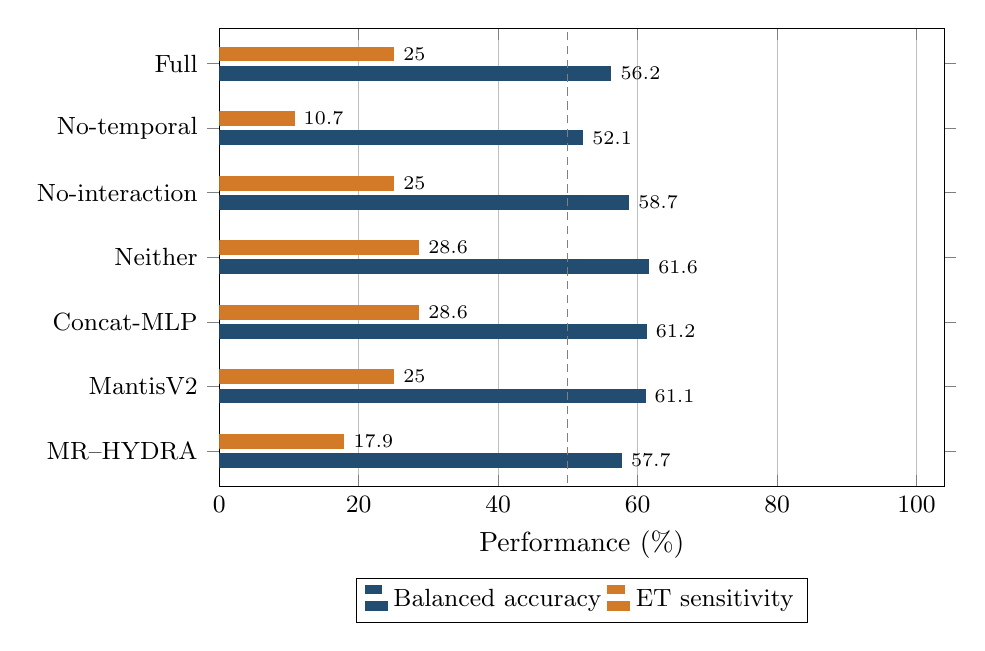
\begin{tikzpicture}
\begin{axis}[width=.89\linewidth,height=7.4cm,xbar,bar width=5pt,
 xmin=0,xmax=104,ymin=.45,ymax=7.55,ytick={1,2,3,4,5,6,7},
 yticklabels={MR--HYDRA,MantisV2,Concat-MLP,Neither,No-interaction,No-temporal,Full},
 xlabel={Performance (\%)},xtick={0,20,40,60,80,100},xmajorgrids,
 tick label style={font=\small},legend style={at={(.5,-.20)},anchor=north,legend columns=2,font=\small},
 nodes near coords,nodes near coords align={horizontal},every node near coord/.append style={font=\scriptsize},
 point meta=x,/pgf/number format/fixed,/pgf/number format/precision=1]
\addplot[fill=navy,draw=navy] coordinates {(56.15942,7) (52.096273,6) (58.695652,5) (61.568323,4) (61.206004,3) (61.050725,2) (57.660455,1)};
\addplot[fill=orangeplot,draw=orangeplot] coordinates {(25,7) (10.714286,6) (25,5) (28.571429,4) (28.571429,3) (25,2) (17.857143,1)};
\draw[densely dashed,gray] (axis cs:50,.5)--(axis cs:50,7.5);
\legend{Balanced accuracy,ET sensitivity}
\end{axis}\end{tikzpicture}
\caption{전체 방법의 외부 BA와 ET 민감도. 점선은 항상 PD로 예측할 때의
BA 50\%다. ET 민감도가 전반적으로 낮고, 전체 모델의 BA가 최고가 아니다.}
\label{fig:bars}
\end{figure}

\subsection{정분류 인원으로 해석한 성능}
\begin{table}[H]\centering\small
\caption{외부 혼동행렬의 인원수. TN/FP의 합은 276명, FN/TP의 합은 28명이다.}
\begin{tabular}{@{}lrrrrr@{}}\toprule
 모델 & TN: PD$\to$PD & FP: PD$\to$ET & FN: ET$\to$PD & TP: ET$\to$ET & ET 예측 수\\\midrule
Full & 241 & 35 & 21 & 7 & 42 \\
No-temporal & 258 & 18 & 25 & 3 & 21 \\
No-interaction & 255 & 21 & 21 & 7 & 28 \\
Neither & 261 & 15 & 20 & 8 & 23 \\
Concat-MLP & 259 & 17 & 20 & 8 & 25 \\
MantisV2 & 268 & 8 & 21 & 7 & 15 \\
MR--HYDRA & 269 & 7 & 23 & 5 & 12 \\
\bottomrule\end{tabular}\label{tab:confusion}
\end{table}
전체 모델은 ET 28명 중 7명을 ET로 분류했고, PD 276명 중 35명을 ET로
오분류하였다. 따라서 ET로 예측한 42명 중 실제 ET는 7명으로,
ET precision은 16.67\%, ET F1은 0.2000이다.

MantisV2도 ET 정분류 인원은 7명이지만 PD 오분류는 8명이다.
두 방법이 맞힌 ET 참가자가 반드시 같은 사람이라는 뜻은 아니다.
전체 모델의 BA가 MantisV2보다 4.89\%p 낮은 것은, 집계상 ET 민감도가 같으면서
PD 정분류 인원이 27명 적은 차이와 일치한다.
MR--HYDRA보다 ET를 2명 더 맞혔지만 PD 정분류 인원은 28명 적어서,
전체 모델의 BA는 오히려 1.50\%p 낮았다.

모든 참가자를 PD로 예측하면 일반 정확도는 $276/304=90.79\%$지만
ET 민감도는 0, BA는 50\%다. 전체 모델의 일반 정확도는 81.58\%이므로,
이 불균형 자료에서 일반 정확도만으로 모델을 선택하면 평가 목적이 달라질 수 있다.

\subsection{순위 구별력과 고정 임계값의 차이}
\begin{figure}[H]\centering
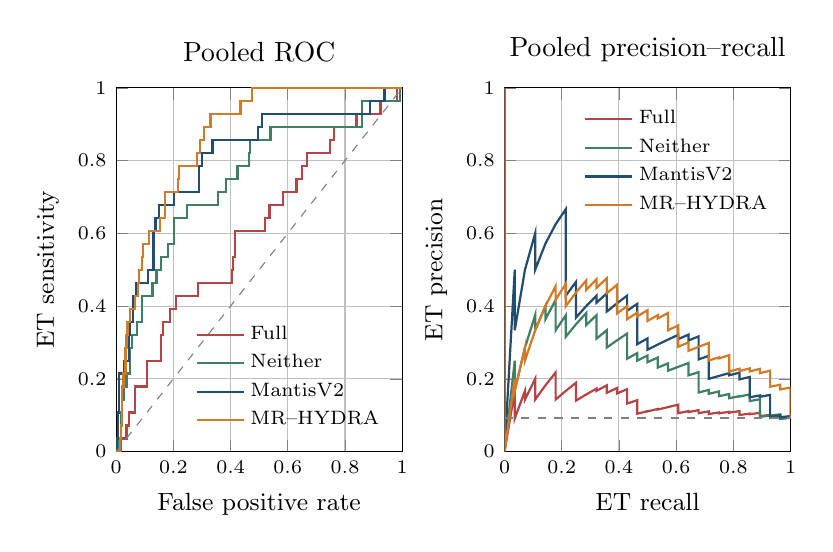
\begin{tikzpicture}\begin{groupplot}[group style={group size=2 by 1,horizontal sep=1.3cm},width=.43\linewidth,height=6.2cm,xmin=0,xmax=1,ymin=0,ymax=1,grid=major,tick label style={font=\scriptsize},label style={font=\small},legend style={font=\scriptsize,draw=none,fill=none},legend cell align=left]
\nextgroupplot[xlabel={False positive rate},ylabel={ET sensitivity},title={Pooled ROC},legend pos=south east]
\addplot[thick,redplot,no marks] coordinates {(0,0) (0.0036231884,0) (0.018115942,0) (0.018115942,0.035714286) (0.036231884,0.035714286) (0.036231884,0.071428571) (0.043478261,0.071428571) (0.043478261,0.10714286) (0.065217391,0.10714286) (0.065217391,0.17857143) (0.10869565,0.17857143) (0.10869565,0.25) (0.1557971,0.25) (0.1557971,0.32142857) (0.16304348,0.32142857) (0.16304348,0.35714286) (0.1884058,0.35714286) (0.1884058,0.39285714) (0.21014493,0.39285714) (0.21014493,0.42857143) (0.28623188,0.42857143) (0.28623188,0.46428571) (0.4057971,0.46428571) (0.4057971,0.5) (0.40942029,0.5) (0.40942029,0.53571429) (0.41666667,0.53571429) (0.41666667,0.60714286) (0.52173913,0.60714286) (0.52173913,0.64285714) (0.53623188,0.64285714) (0.53623188,0.67857143) (0.58333333,0.67857143) (0.58333333,0.71428571) (0.63043478,0.71428571) (0.63043478,0.75) (0.64855072,0.75) (0.64855072,0.78571429) (0.66666667,0.78571429) (0.66666667,0.82142857) (0.74637681,0.82142857) (0.74637681,0.85714286) (0.76086957,0.85714286) (0.76086957,0.89285714) (0.84057971,0.89285714) (0.84057971,0.92857143) (0.92391304,0.92857143) (0.92391304,0.96428571) (0.98188406,0.96428571) (0.98188406,1) (1,1)};
\addlegendentry{Full}
\addplot[thick,greenplot,no marks] coordinates {(0,0) (0.0036231884,0) (0.010869565,0) (0.010869565,0.035714286) (0.018115942,0.035714286) (0.018115942,0.10714286) (0.02173913,0.10714286) (0.02173913,0.14285714) (0.025362319,0.14285714) (0.025362319,0.17857143) (0.036231884,0.17857143) (0.036231884,0.21428571) (0.047101449,0.21428571) (0.047101449,0.28571429) (0.054347826,0.28571429) (0.054347826,0.32142857) (0.072463768,0.32142857) (0.072463768,0.35714286) (0.09057971,0.35714286) (0.09057971,0.42857143) (0.12681159,0.42857143) (0.12681159,0.46428571) (0.14130435,0.46428571) (0.14130435,0.5) (0.1557971,0.5) (0.1557971,0.53571429) (0.18115942,0.53571429) (0.18115942,0.57142857) (0.20289855,0.57142857) (0.20289855,0.64285714) (0.24637681,0.64285714) (0.24637681,0.67857143) (0.35507246,0.67857143) (0.35507246,0.71428571) (0.38405797,0.71428571) (0.38405797,0.75) (0.42391304,0.75) (0.42391304,0.78571429) (0.46376812,0.78571429) (0.46376812,0.82142857) (0.4673913,0.82142857) (0.4673913,0.85714286) (0.53985507,0.85714286) (0.53985507,0.89285714) (0.85869565,0.89285714) (0.85869565,0.96428571) (0.99275362,0.96428571) (0.99275362,1) (1,1)};
\addlegendentry{Neither}
\addplot[thick,navy,no marks] coordinates {(0,0) (0.0036231884,0) (0.0036231884,0.035714286) (0.0072463768,0.035714286) (0.0072463768,0.10714286) (0.010869565,0.10714286) (0.010869565,0.21428571) (0.028985507,0.21428571) (0.028985507,0.25) (0.043478261,0.25) (0.043478261,0.32142857) (0.047101449,0.32142857) (0.047101449,0.35714286) (0.057971014,0.35714286) (0.057971014,0.42857143) (0.06884058,0.42857143) (0.06884058,0.46428571) (0.11231884,0.46428571) (0.11231884,0.5) (0.13043478,0.5) (0.13043478,0.60714286) (0.13768116,0.60714286) (0.13768116,0.64285714) (0.14855072,0.64285714) (0.14855072,0.67857143) (0.20289855,0.67857143) (0.20289855,0.71428571) (0.28985507,0.71428571) (0.28985507,0.78571429) (0.30072464,0.78571429) (0.30072464,0.82142857) (0.33695652,0.82142857) (0.33695652,0.85714286) (0.49637681,0.85714286) (0.49637681,0.89285714) (0.51086957,0.89285714) (0.51086957,0.92857143) (0.88768116,0.92857143) (0.88768116,0.96428571) (0.9384058,0.96428571) (0.9384058,1) (1,1)};
\addlegendentry{MantisV2}
\addplot[thick,orangeplot,no marks] coordinates {(0,0) (0.0036231884,0) (0.014492754,0) (0.014492754,0.035714286) (0.018115942,0.035714286) (0.018115942,0.071428571) (0.02173913,0.071428571) (0.02173913,0.17857143) (0.025362319,0.17857143) (0.025362319,0.21428571) (0.032608696,0.21428571) (0.032608696,0.28571429) (0.036231884,0.28571429) (0.036231884,0.32142857) (0.039855072,0.32142857) (0.039855072,0.35714286) (0.047101449,0.35714286) (0.047101449,0.39285714) (0.065217391,0.39285714) (0.065217391,0.42857143) (0.076086957,0.42857143) (0.076086957,0.46428571) (0.079710145,0.46428571) (0.079710145,0.5) (0.09057971,0.5) (0.09057971,0.53571429) (0.094202899,0.53571429) (0.094202899,0.57142857) (0.11594203,0.57142857) (0.11594203,0.60714286) (0.15217391,0.60714286) (0.15217391,0.64285714) (0.17028986,0.64285714) (0.17028986,0.71428571) (0.2173913,0.71428571) (0.2173913,0.75) (0.22101449,0.75) (0.22101449,0.78571429) (0.2826087,0.78571429) (0.2826087,0.82142857) (0.29347826,0.82142857) (0.29347826,0.85714286) (0.30797101,0.85714286) (0.30797101,0.89285714) (0.32971014,0.89285714) (0.32971014,0.92857143) (0.43478261,0.92857143) (0.43478261,0.96428571) (0.47463768,0.96428571) (0.47463768,1) (1,1)};
\addlegendentry{MR--HYDRA}
\addplot[dashed,gray,forget plot] coordinates {(0,0)(1,1)};
\nextgroupplot[xlabel={ET recall},ylabel={ET precision},title={Pooled precision--recall},legend pos=north east]
\addplot[thick,redplot,no marks] coordinates {(1,0.092105263) (1,0.092409241) (1,0.092715232) (1,0.093023256) (1,0.093333333) (1,0.093645485) (0.96428571,0.090604027) (0.96428571,0.090909091) (0.96428571,0.091216216) (0.96428571,0.091525424) (0.96428571,0.091836735) (0.96428571,0.092150171) (0.96428571,0.092465753) (0.96428571,0.092783505) (0.96428571,0.093103448) (0.96428571,0.093425606) (0.96428571,0.09375) (0.96428571,0.094076655) (0.96428571,0.094405594) (0.96428571,0.094736842) (0.96428571,0.095070423) (0.96428571,0.09540636) (0.96428571,0.095744681) (0.92857143,0.09252669) (0.92857143,0.092857143) (0.92857143,0.093189964) (0.92857143,0.09352518) (0.92857143,0.093862816) (0.92857143,0.094202899) (0.92857143,0.094545455) (0.92857143,0.094890511) (0.92857143,0.095238095) (0.92857143,0.095588235) (0.92857143,0.095940959) (0.92857143,0.096296296) (0.92857143,0.096654275) (0.92857143,0.097014925) (0.92857143,0.097378277) (0.92857143,0.097744361) (0.92857143,0.098113208) (0.92857143,0.098484848) (0.92857143,0.098859316) (0.92857143,0.099236641) (0.92857143,0.099616858) (0.92857143,0.1) (0.92857143,0.1003861) (0.92857143,0.10077519) (0.89285714,0.097276265) (0.89285714,0.09765625) (0.89285714,0.098039216) (0.89285714,0.098425197) (0.89285714,0.098814229) (0.89285714,0.099206349) (0.89285714,0.099601594) (0.89285714,0.1) (0.89285714,0.10040161) (0.89285714,0.10080645) (0.89285714,0.10121457) (0.89285714,0.10162602) (0.89285714,0.10204082) (0.89285714,0.10245902) (0.89285714,0.10288066) (0.89285714,0.10330579) (0.89285714,0.10373444) (0.89285714,0.10416667) (0.89285714,0.10460251) (0.89285714,0.10504202) (0.89285714,0.10548523) (0.89285714,0.1059322) (0.89285714,0.10638298) (0.85714286,0.1025641) (0.85714286,0.10300429) (0.85714286,0.10344828) (0.85714286,0.1038961) (0.85714286,0.10434783) (0.82142857,0.10043668) (0.82142857,0.10087719) (0.82142857,0.10132159) (0.82142857,0.10176991) (0.82142857,0.10222222) (0.82142857,0.10267857) (0.82142857,0.10313901) (0.82142857,0.1036036) (0.82142857,0.1040724) (0.82142857,0.10454545) (0.82142857,0.10502283) (0.82142857,0.10550459) (0.82142857,0.10599078) (0.82142857,0.10648148) (0.82142857,0.10697674) (0.82142857,0.10747664) (0.82142857,0.10798122) (0.82142857,0.10849057) (0.82142857,0.10900474) (0.82142857,0.10952381) (0.82142857,0.11004785) (0.82142857,0.11057692) (0.82142857,0.11111111) (0.78571429,0.10679612) (0.78571429,0.10731707) (0.78571429,0.10784314) (0.78571429,0.10837438) (0.78571429,0.10891089) (0.78571429,0.10945274) (0.75,0.105) (0.75,0.10552764) (0.75,0.10606061) (0.75,0.10659898) (0.75,0.10714286) (0.75,0.10769231) (0.71428571,0.10309278) (0.71428571,0.10362694) (0.71428571,0.10416667) (0.71428571,0.10471204) (0.71428571,0.10526316) (0.71428571,0.10582011) (0.71428571,0.10638298) (0.71428571,0.10695187) (0.71428571,0.10752688) (0.71428571,0.10810811) (0.71428571,0.10869565) (0.71428571,0.10928962) (0.71428571,0.10989011) (0.71428571,0.11049724) (0.67857143,0.10555556) (0.67857143,0.10614525) (0.67857143,0.10674157) (0.67857143,0.10734463) (0.67857143,0.10795455) (0.67857143,0.10857143) (0.67857143,0.1091954) (0.67857143,0.10982659) (0.67857143,0.11046512) (0.67857143,0.11111111) (0.67857143,0.11176471) (0.67857143,0.11242604) (0.67857143,0.11309524) (0.67857143,0.11377246) (0.64285714,0.10843373) (0.64285714,0.10909091) (0.64285714,0.1097561) (0.64285714,0.11042945) (0.64285714,0.11111111) (0.60714286,0.10559006) (0.60714286,0.10625) (0.60714286,0.10691824) (0.60714286,0.10759494) (0.60714286,0.10828025) (0.60714286,0.10897436) (0.60714286,0.10967742) (0.60714286,0.11038961) (0.60714286,0.11111111) (0.60714286,0.11184211) (0.60714286,0.11258278) (0.60714286,0.11333333) (0.60714286,0.11409396) (0.60714286,0.11486486) (0.60714286,0.11564626) (0.60714286,0.11643836) (0.60714286,0.11724138) (0.60714286,0.11805556) (0.60714286,0.11888112) (0.60714286,0.11971831) (0.60714286,0.12056738) (0.60714286,0.12142857) (0.60714286,0.12230216) (0.60714286,0.12318841) (0.60714286,0.12408759) (0.60714286,0.125) (0.60714286,0.12592593) (0.60714286,0.12686567) (0.60714286,0.12781955) (0.60714286,0.12878788) (0.57142857,0.1221374) (0.53571429,0.11538462) (0.53571429,0.11627907) (0.53571429,0.1171875) (0.5,0.11023622) (0.5,0.11111111) (0.46428571,0.104) (0.46428571,0.10483871) (0.46428571,0.10569106) (0.46428571,0.10655738) (0.46428571,0.10743802) (0.46428571,0.10833333) (0.46428571,0.1092437) (0.46428571,0.11016949) (0.46428571,0.11111111) (0.46428571,0.11206897) (0.46428571,0.11304348) (0.46428571,0.11403509) (0.46428571,0.11504425) (0.46428571,0.11607143) (0.46428571,0.11711712) (0.46428571,0.11818182) (0.46428571,0.11926606) (0.46428571,0.12037037) (0.46428571,0.12149533) (0.46428571,0.12264151) (0.46428571,0.12380952) (0.46428571,0.125) (0.46428571,0.12621359) (0.46428571,0.12745098) (0.46428571,0.12871287) (0.46428571,0.13) (0.46428571,0.13131313) (0.46428571,0.13265306) (0.46428571,0.13402062) (0.46428571,0.13541667) (0.46428571,0.13684211) (0.46428571,0.13829787) (0.46428571,0.13978495) (0.46428571,0.14130435) (0.42857143,0.13186813) (0.42857143,0.13333333) (0.42857143,0.13483146) (0.42857143,0.13636364) (0.42857143,0.13793103) (0.42857143,0.13953488) (0.42857143,0.14117647) (0.42857143,0.14285714) (0.42857143,0.14457831) (0.42857143,0.14634146) (0.42857143,0.14814815) (0.42857143,0.15) (0.42857143,0.15189873) (0.42857143,0.15384615) (0.42857143,0.15584416) (0.42857143,0.15789474) (0.42857143,0.16) (0.42857143,0.16216216) (0.42857143,0.16438356) (0.42857143,0.16666667) (0.42857143,0.16901408) (0.42857143,0.17142857) (0.39285714,0.15942029) (0.39285714,0.16176471) (0.39285714,0.1641791) (0.39285714,0.16666667) (0.39285714,0.16923077) (0.39285714,0.171875) (0.39285714,0.17460317) (0.35714286,0.16129032) (0.35714286,0.16393443) (0.35714286,0.16666667) (0.35714286,0.16949153) (0.35714286,0.17241379) (0.35714286,0.1754386) (0.35714286,0.17857143) (0.35714286,0.18181818) (0.32142857,0.16666667) (0.32142857,0.16981132) (0.32142857,0.17307692) (0.28571429,0.15686275) (0.25,0.14) (0.25,0.14285714) (0.25,0.14583333) (0.25,0.14893617) (0.25,0.15217391) (0.25,0.15555556) (0.25,0.15909091) (0.25,0.1627907) (0.25,0.16666667) (0.25,0.17073171) (0.25,0.175) (0.25,0.17948718) (0.25,0.18421053) (0.25,0.18918919) (0.21428571,0.16666667) (0.17857143,0.14285714) (0.17857143,0.14705882) (0.17857143,0.15151515) (0.17857143,0.15625) (0.17857143,0.16129032) (0.17857143,0.16666667) (0.17857143,0.17241379) (0.17857143,0.17857143) (0.17857143,0.18518519) (0.17857143,0.19230769) (0.17857143,0.2) (0.17857143,0.20833333) (0.17857143,0.2173913) (0.14285714,0.18181818) (0.10714286,0.14285714) (0.10714286,0.15) (0.10714286,0.15789474) (0.10714286,0.16666667) (0.10714286,0.17647059) (0.10714286,0.1875) (0.10714286,0.2) (0.071428571,0.14285714) (0.071428571,0.15384615) (0.071428571,0.16666667) (0.035714286,0.090909091) (0.035714286,0.1) (0.035714286,0.11111111) (0.035714286,0.125) (0.035714286,0.14285714) (0.035714286,0.16666667) (0,0) (0,0) (0,0) (0,0) (0,0) (0,1)};
\addlegendentry{Full}
\addplot[thick,greenplot,no marks] coordinates {(1,0.092105263) (1,0.092409241) (1,0.092715232) (0.96428571,0.089700997) (0.96428571,0.09) (0.96428571,0.090301003) (0.96428571,0.090604027) (0.96428571,0.090909091) (0.96428571,0.091216216) (0.96428571,0.091525424) (0.96428571,0.091836735) (0.96428571,0.092150171) (0.96428571,0.092465753) (0.96428571,0.092783505) (0.96428571,0.093103448) (0.96428571,0.093425606) (0.96428571,0.09375) (0.96428571,0.094076655) (0.96428571,0.094405594) (0.96428571,0.094736842) (0.96428571,0.095070423) (0.96428571,0.09540636) (0.96428571,0.095744681) (0.96428571,0.096085409) (0.96428571,0.096428571) (0.96428571,0.096774194) (0.96428571,0.097122302) (0.96428571,0.097472924) (0.96428571,0.097826087) (0.96428571,0.098181818) (0.96428571,0.098540146) (0.96428571,0.098901099) (0.96428571,0.099264706) (0.96428571,0.099630996) (0.96428571,0.1) (0.96428571,0.10037175) (0.96428571,0.10074627) (0.96428571,0.1011236) (0.96428571,0.10150376) (0.96428571,0.10188679) (0.96428571,0.10227273) (0.92857143,0.098859316) (0.89285714,0.095419847) (0.89285714,0.095785441) (0.89285714,0.096153846) (0.89285714,0.096525097) (0.89285714,0.096899225) (0.89285714,0.097276265) (0.89285714,0.09765625) (0.89285714,0.098039216) (0.89285714,0.098425197) (0.89285714,0.098814229) (0.89285714,0.099206349) (0.89285714,0.099601594) (0.89285714,0.1) (0.89285714,0.10040161) (0.89285714,0.10080645) (0.89285714,0.10121457) (0.89285714,0.10162602) (0.89285714,0.10204082) (0.89285714,0.10245902) (0.89285714,0.10288066) (0.89285714,0.10330579) (0.89285714,0.10373444) (0.89285714,0.10416667) (0.89285714,0.10460251) (0.89285714,0.10504202) (0.89285714,0.10548523) (0.89285714,0.1059322) (0.89285714,0.10638298) (0.89285714,0.10683761) (0.89285714,0.10729614) (0.89285714,0.10775862) (0.89285714,0.10822511) (0.89285714,0.10869565) (0.89285714,0.10917031) (0.89285714,0.10964912) (0.89285714,0.11013216) (0.89285714,0.11061947) (0.89285714,0.11111111) (0.89285714,0.11160714) (0.89285714,0.11210762) (0.89285714,0.11261261) (0.89285714,0.11312217) (0.89285714,0.11363636) (0.89285714,0.11415525) (0.89285714,0.1146789) (0.89285714,0.11520737) (0.89285714,0.11574074) (0.89285714,0.11627907) (0.89285714,0.11682243) (0.89285714,0.11737089) (0.89285714,0.11792453) (0.89285714,0.11848341) (0.89285714,0.11904762) (0.89285714,0.11961722) (0.89285714,0.12019231) (0.89285714,0.12077295) (0.89285714,0.12135922) (0.89285714,0.12195122) (0.89285714,0.12254902) (0.89285714,0.12315271) (0.89285714,0.12376238) (0.89285714,0.12437811) (0.89285714,0.125) (0.89285714,0.12562814) (0.89285714,0.12626263) (0.89285714,0.12690355) (0.89285714,0.12755102) (0.89285714,0.12820513) (0.89285714,0.12886598) (0.89285714,0.12953368) (0.89285714,0.13020833) (0.89285714,0.13089005) (0.89285714,0.13157895) (0.89285714,0.13227513) (0.89285714,0.13297872) (0.89285714,0.13368984) (0.89285714,0.1344086) (0.89285714,0.13513514) (0.89285714,0.13586957) (0.89285714,0.13661202) (0.89285714,0.13736264) (0.89285714,0.13812155) (0.89285714,0.13888889) (0.89285714,0.1396648) (0.89285714,0.14044944) (0.89285714,0.14124294) (0.89285714,0.14204545) (0.89285714,0.14285714) (0.89285714,0.14367816) (0.85714286,0.13872832) (0.85714286,0.13953488) (0.85714286,0.14035088) (0.85714286,0.14117647) (0.85714286,0.14201183) (0.85714286,0.14285714) (0.85714286,0.14371257) (0.85714286,0.14457831) (0.85714286,0.14545455) (0.85714286,0.14634146) (0.85714286,0.14723926) (0.85714286,0.14814815) (0.85714286,0.14906832) (0.85714286,0.15) (0.85714286,0.1509434) (0.85714286,0.15189873) (0.85714286,0.15286624) (0.85714286,0.15384615) (0.85714286,0.15483871) (0.85714286,0.15584416) (0.85714286,0.15686275) (0.82142857,0.15131579) (0.82142857,0.15231788) (0.78571429,0.14666667) (0.78571429,0.14765101) (0.78571429,0.14864865) (0.78571429,0.14965986) (0.78571429,0.15068493) (0.78571429,0.15172414) (0.78571429,0.15277778) (0.78571429,0.15384615) (0.78571429,0.15492958) (0.78571429,0.15602837) (0.78571429,0.15714286) (0.78571429,0.15827338) (0.75,0.15217391) (0.75,0.15328467) (0.75,0.15441176) (0.75,0.15555556) (0.75,0.15671642) (0.75,0.15789474) (0.75,0.15909091) (0.75,0.16030534) (0.75,0.16153846) (0.75,0.1627907) (0.75,0.1640625) (0.75,0.16535433) (0.71428571,0.15873016) (0.71428571,0.16) (0.71428571,0.16129032) (0.71428571,0.16260163) (0.71428571,0.16393443) (0.71428571,0.16528926) (0.71428571,0.16666667) (0.71428571,0.16806723) (0.71428571,0.16949153) (0.67857143,0.16239316) (0.67857143,0.1637931) (0.67857143,0.16521739) (0.67857143,0.16666667) (0.67857143,0.16814159) (0.67857143,0.16964286) (0.67857143,0.17117117) (0.67857143,0.17272727) (0.67857143,0.17431193) (0.67857143,0.17592593) (0.67857143,0.17757009) (0.67857143,0.17924528) (0.67857143,0.18095238) (0.67857143,0.18269231) (0.67857143,0.18446602) (0.67857143,0.18627451) (0.67857143,0.18811881) (0.67857143,0.19) (0.67857143,0.19191919) (0.67857143,0.19387755) (0.67857143,0.19587629) (0.67857143,0.19791667) (0.67857143,0.2) (0.67857143,0.20212766) (0.67857143,0.20430108) (0.67857143,0.20652174) (0.67857143,0.20879121) (0.67857143,0.21111111) (0.67857143,0.21348315) (0.67857143,0.21590909) (0.67857143,0.2183908) (0.64285714,0.20930233) (0.64285714,0.21176471) (0.64285714,0.21428571) (0.64285714,0.21686747) (0.64285714,0.2195122) (0.64285714,0.22222222) (0.64285714,0.225) (0.64285714,0.2278481) (0.64285714,0.23076923) (0.64285714,0.23376623) (0.64285714,0.23684211) (0.64285714,0.24) (0.64285714,0.24324324) (0.60714286,0.23287671) (0.57142857,0.22222222) (0.57142857,0.22535211) (0.57142857,0.22857143) (0.57142857,0.23188406) (0.57142857,0.23529412) (0.57142857,0.23880597) (0.57142857,0.24242424) (0.53571429,0.23076923) (0.53571429,0.234375) (0.53571429,0.23809524) (0.53571429,0.24193548) (0.53571429,0.24590164) (0.53571429,0.25) (0.53571429,0.25423729) (0.53571429,0.25862069) (0.5,0.24561404) (0.5,0.25) (0.5,0.25454545) (0.5,0.25925926) (0.5,0.26415094) (0.46428571,0.25) (0.46428571,0.25490196) (0.46428571,0.26) (0.46428571,0.26530612) (0.46428571,0.27083333) (0.42857143,0.25531915) (0.42857143,0.26086957) (0.42857143,0.26666667) (0.42857143,0.27272727) (0.42857143,0.27906977) (0.42857143,0.28571429) (0.42857143,0.29268293) (0.42857143,0.3) (0.42857143,0.30769231) (0.42857143,0.31578947) (0.42857143,0.32432432) (0.39285714,0.30555556) (0.35714286,0.28571429) (0.35714286,0.29411765) (0.35714286,0.3030303) (0.35714286,0.3125) (0.35714286,0.32258065) (0.35714286,0.33333333) (0.32142857,0.31034483) (0.32142857,0.32142857) (0.32142857,0.33333333) (0.32142857,0.34615385) (0.32142857,0.36) (0.32142857,0.375) (0.28571429,0.34782609) (0.28571429,0.36363636) (0.28571429,0.38095238) (0.25,0.35) (0.21428571,0.31578947) (0.21428571,0.33333333) (0.21428571,0.35294118) (0.21428571,0.375) (0.17857143,0.33333333) (0.17857143,0.35714286) (0.17857143,0.38461538) (0.17857143,0.41666667) (0.14285714,0.36363636) (0.14285714,0.4) (0.10714286,0.33333333) (0.10714286,0.375) (0.071428571,0.28571429) (0.035714286,0.16666667) (0.035714286,0.2) (0.035714286,0.25) (0,0) (0,0) (0,0) (0,1)};
\addlegendentry{Neither}
\addplot[thick,navy,no marks] coordinates {(1,0.092105263) (1,0.092409241) (1,0.092715232) (1,0.093023256) (1,0.093333333) (1,0.093645485) (1,0.093959732) (1,0.094276094) (1,0.094594595) (1,0.094915254) (1,0.095238095) (1,0.09556314) (1,0.095890411) (1,0.096219931) (1,0.096551724) (1,0.096885813) (1,0.097222222) (1,0.097560976) (0.96428571,0.094405594) (0.96428571,0.094736842) (0.96428571,0.095070423) (0.96428571,0.09540636) (0.96428571,0.095744681) (0.96428571,0.096085409) (0.96428571,0.096428571) (0.96428571,0.096774194) (0.96428571,0.097122302) (0.96428571,0.097472924) (0.96428571,0.097826087) (0.96428571,0.098181818) (0.96428571,0.098540146) (0.96428571,0.098901099) (0.96428571,0.099264706) (0.92857143,0.095940959) (0.92857143,0.096296296) (0.92857143,0.096654275) (0.92857143,0.097014925) (0.92857143,0.097378277) (0.92857143,0.097744361) (0.92857143,0.098113208) (0.92857143,0.098484848) (0.92857143,0.098859316) (0.92857143,0.099236641) (0.92857143,0.099616858) (0.92857143,0.1) (0.92857143,0.1003861) (0.92857143,0.10077519) (0.92857143,0.10116732) (0.92857143,0.1015625) (0.92857143,0.10196078) (0.92857143,0.1023622) (0.92857143,0.1027668) (0.92857143,0.1031746) (0.92857143,0.10358566) (0.92857143,0.104) (0.92857143,0.10441767) (0.92857143,0.10483871) (0.92857143,0.10526316) (0.92857143,0.10569106) (0.92857143,0.10612245) (0.92857143,0.10655738) (0.92857143,0.10699588) (0.92857143,0.10743802) (0.92857143,0.10788382) (0.92857143,0.10833333) (0.92857143,0.10878661) (0.92857143,0.1092437) (0.92857143,0.10970464) (0.92857143,0.11016949) (0.92857143,0.1106383) (0.92857143,0.11111111) (0.92857143,0.11158798) (0.92857143,0.11206897) (0.92857143,0.11255411) (0.92857143,0.11304348) (0.92857143,0.11353712) (0.92857143,0.11403509) (0.92857143,0.11453744) (0.92857143,0.11504425) (0.92857143,0.11555556) (0.92857143,0.11607143) (0.92857143,0.11659193) (0.92857143,0.11711712) (0.92857143,0.11764706) (0.92857143,0.11818182) (0.92857143,0.11872146) (0.92857143,0.11926606) (0.92857143,0.11981567) (0.92857143,0.12037037) (0.92857143,0.12093023) (0.92857143,0.12149533) (0.92857143,0.12206573) (0.92857143,0.12264151) (0.92857143,0.12322275) (0.92857143,0.12380952) (0.92857143,0.12440191) (0.92857143,0.125) (0.92857143,0.12560386) (0.92857143,0.12621359) (0.92857143,0.12682927) (0.92857143,0.12745098) (0.92857143,0.12807882) (0.92857143,0.12871287) (0.92857143,0.12935323) (0.92857143,0.13) (0.92857143,0.13065327) (0.92857143,0.13131313) (0.92857143,0.1319797) (0.92857143,0.13265306) (0.92857143,0.13333333) (0.92857143,0.13402062) (0.92857143,0.13471503) (0.92857143,0.13541667) (0.92857143,0.13612565) (0.92857143,0.13684211) (0.92857143,0.13756614) (0.92857143,0.13829787) (0.92857143,0.13903743) (0.92857143,0.13978495) (0.92857143,0.14054054) (0.92857143,0.14130435) (0.92857143,0.1420765) (0.92857143,0.14285714) (0.92857143,0.14364641) (0.92857143,0.14444444) (0.92857143,0.1452514) (0.92857143,0.14606742) (0.92857143,0.14689266) (0.92857143,0.14772727) (0.92857143,0.14857143) (0.92857143,0.14942529) (0.92857143,0.15028902) (0.92857143,0.15116279) (0.92857143,0.15204678) (0.92857143,0.15294118) (0.92857143,0.15384615) (0.92857143,0.1547619) (0.92857143,0.15568862) (0.89285714,0.15060241) (0.89285714,0.15151515) (0.89285714,0.15243902) (0.89285714,0.15337423) (0.89285714,0.15432099) (0.85714286,0.14906832) (0.85714286,0.15) (0.85714286,0.1509434) (0.85714286,0.15189873) (0.85714286,0.15286624) (0.85714286,0.15384615) (0.85714286,0.15483871) (0.85714286,0.15584416) (0.85714286,0.15686275) (0.85714286,0.15789474) (0.85714286,0.1589404) (0.85714286,0.16) (0.85714286,0.16107383) (0.85714286,0.16216216) (0.85714286,0.16326531) (0.85714286,0.16438356) (0.85714286,0.16551724) (0.85714286,0.16666667) (0.85714286,0.16783217) (0.85714286,0.16901408) (0.85714286,0.17021277) (0.85714286,0.17142857) (0.85714286,0.17266187) (0.85714286,0.17391304) (0.85714286,0.17518248) (0.85714286,0.17647059) (0.85714286,0.17777778) (0.85714286,0.17910448) (0.85714286,0.18045113) (0.85714286,0.18181818) (0.85714286,0.18320611) (0.85714286,0.18461538) (0.85714286,0.18604651) (0.85714286,0.1875) (0.85714286,0.18897638) (0.85714286,0.19047619) (0.85714286,0.192) (0.85714286,0.19354839) (0.85714286,0.19512195) (0.85714286,0.19672131) (0.85714286,0.19834711) (0.85714286,0.2) (0.85714286,0.20168067) (0.85714286,0.20338983) (0.85714286,0.20512821) (0.82142857,0.19827586) (0.82142857,0.2) (0.82142857,0.20175439) (0.82142857,0.20353982) (0.82142857,0.20535714) (0.82142857,0.20720721) (0.82142857,0.20909091) (0.82142857,0.21100917) (0.82142857,0.21296296) (0.82142857,0.21495327) (0.82142857,0.21698113) (0.78571429,0.20952381) (0.78571429,0.21153846) (0.78571429,0.21359223) (0.78571429,0.21568627) (0.75,0.20792079) (0.71428571,0.2) (0.71428571,0.2020202) (0.71428571,0.20408163) (0.71428571,0.20618557) (0.71428571,0.20833333) (0.71428571,0.21052632) (0.71428571,0.21276596) (0.71428571,0.21505376) (0.71428571,0.2173913) (0.71428571,0.21978022) (0.71428571,0.22222222) (0.71428571,0.2247191) (0.71428571,0.22727273) (0.71428571,0.22988506) (0.71428571,0.23255814) (0.71428571,0.23529412) (0.71428571,0.23809524) (0.71428571,0.24096386) (0.71428571,0.24390244) (0.71428571,0.24691358) (0.71428571,0.25) (0.71428571,0.25316456) (0.71428571,0.25641026) (0.71428571,0.25974026) (0.71428571,0.26315789) (0.67857143,0.25333333) (0.67857143,0.25675676) (0.67857143,0.26027397) (0.67857143,0.26388889) (0.67857143,0.26760563) (0.67857143,0.27142857) (0.67857143,0.27536232) (0.67857143,0.27941176) (0.67857143,0.28358209) (0.67857143,0.28787879) (0.67857143,0.29230769) (0.67857143,0.296875) (0.67857143,0.3015873) (0.67857143,0.30645161) (0.67857143,0.31147541) (0.67857143,0.31666667) (0.64285714,0.30508475) (0.64285714,0.31034483) (0.64285714,0.31578947) (0.64285714,0.32142857) (0.60714286,0.30909091) (0.60714286,0.31481481) (0.60714286,0.32075472) (0.57142857,0.30769231) (0.53571429,0.29411765) (0.5,0.28) (0.5,0.28571429) (0.5,0.29166667) (0.5,0.29787234) (0.5,0.30434783) (0.5,0.31111111) (0.46428571,0.29545455) (0.46428571,0.30232558) (0.46428571,0.30952381) (0.46428571,0.31707317) (0.46428571,0.325) (0.46428571,0.33333333) (0.46428571,0.34210526) (0.46428571,0.35135135) (0.46428571,0.36111111) (0.46428571,0.37142857) (0.46428571,0.38235294) (0.46428571,0.39393939) (0.46428571,0.40625) (0.42857143,0.38709677) (0.42857143,0.4) (0.42857143,0.4137931) (0.42857143,0.42857143) (0.39285714,0.40740741) (0.35714286,0.38461538) (0.35714286,0.4) (0.35714286,0.41666667) (0.35714286,0.43478261) (0.32142857,0.40909091) (0.32142857,0.42857143) (0.28571429,0.4) (0.25,0.36842105) (0.25,0.38888889) (0.25,0.41176471) (0.25,0.4375) (0.25,0.46666667) (0.21428571,0.42857143) (0.21428571,0.46153846) (0.21428571,0.5) (0.21428571,0.54545455) (0.21428571,0.6) (0.21428571,0.66666667) (0.17857143,0.625) (0.14285714,0.57142857) (0.10714286,0.5) (0.10714286,0.6) (0.071428571,0.5) (0.035714286,0.33333333) (0.035714286,0.5) (0,0) (0,1)};
\addlegendentry{MantisV2}
\addplot[thick,orangeplot,no marks] coordinates {(1,0.092105263) (1,0.092409241) (1,0.092715232) (1,0.093023256) (1,0.093333333) (1,0.093645485) (1,0.093959732) (1,0.094276094) (1,0.094594595) (1,0.094915254) (1,0.095238095) (1,0.09556314) (1,0.095890411) (1,0.096219931) (1,0.096551724) (1,0.096885813) (1,0.097222222) (1,0.097560976) (1,0.097902098) (1,0.098245614) (1,0.098591549) (1,0.098939929) (1,0.09929078) (1,0.099644128) (1,0.1) (1,0.10035842) (1,0.10071942) (1,0.10108303) (1,0.10144928) (1,0.10181818) (1,0.10218978) (1,0.1025641) (1,0.10294118) (1,0.10332103) (1,0.1037037) (1,0.10408922) (1,0.10447761) (1,0.10486891) (1,0.10526316) (1,0.10566038) (1,0.10606061) (1,0.10646388) (1,0.10687023) (1,0.10727969) (1,0.10769231) (1,0.10810811) (1,0.10852713) (1,0.10894942) (1,0.109375) (1,0.10980392) (1,0.11023622) (1,0.11067194) (1,0.11111111) (1,0.11155378) (1,0.112) (1,0.1124498) (1,0.11290323) (1,0.11336032) (1,0.11382114) (1,0.11428571) (1,0.1147541) (1,0.11522634) (1,0.11570248) (1,0.11618257) (1,0.11666667) (1,0.11715481) (1,0.11764706) (1,0.11814346) (1,0.11864407) (1,0.11914894) (1,0.11965812) (1,0.12017167) (1,0.12068966) (1,0.12121212) (1,0.12173913) (1,0.12227074) (1,0.12280702) (1,0.12334802) (1,0.12389381) (1,0.12444444) (1,0.125) (1,0.12556054) (1,0.12612613) (1,0.12669683) (1,0.12727273) (1,0.12785388) (1,0.12844037) (1,0.12903226) (1,0.12962963) (1,0.13023256) (1,0.13084112) (1,0.1314554) (1,0.13207547) (1,0.13270142) (1,0.13333333) (1,0.13397129) (1,0.13461538) (1,0.1352657) (1,0.13592233) (1,0.13658537) (1,0.1372549) (1,0.13793103) (1,0.13861386) (1,0.13930348) (1,0.14) (1,0.14070352) (1,0.14141414) (1,0.14213198) (1,0.14285714) (1,0.14358974) (1,0.1443299) (1,0.14507772) (1,0.14583333) (1,0.14659686) (1,0.14736842) (1,0.14814815) (1,0.14893617) (1,0.14973262) (1,0.15053763) (1,0.15135135) (1,0.15217391) (1,0.15300546) (1,0.15384615) (1,0.15469613) (1,0.15555556) (1,0.15642458) (1,0.15730337) (1,0.15819209) (1,0.15909091) (1,0.16) (1,0.16091954) (1,0.16184971) (1,0.1627907) (1,0.16374269) (1,0.16470588) (1,0.16568047) (1,0.16666667) (1,0.16766467) (1,0.1686747) (1,0.16969697) (1,0.17073171) (1,0.17177914) (1,0.17283951) (1,0.17391304) (1,0.175) (1,0.17610063) (0.96428571,0.17088608) (0.96428571,0.17197452) (0.96428571,0.17307692) (0.96428571,0.17419355) (0.96428571,0.17532468) (0.96428571,0.17647059) (0.96428571,0.17763158) (0.96428571,0.17880795) (0.96428571,0.18) (0.96428571,0.18120805) (0.96428571,0.18243243) (0.96428571,0.18367347) (0.92857143,0.17808219) (0.92857143,0.17931034) (0.92857143,0.18055556) (0.92857143,0.18181818) (0.92857143,0.18309859) (0.92857143,0.18439716) (0.92857143,0.18571429) (0.92857143,0.18705036) (0.92857143,0.1884058) (0.92857143,0.18978102) (0.92857143,0.19117647) (0.92857143,0.19259259) (0.92857143,0.19402985) (0.92857143,0.19548872) (0.92857143,0.1969697) (0.92857143,0.19847328) (0.92857143,0.2) (0.92857143,0.20155039) (0.92857143,0.203125) (0.92857143,0.20472441) (0.92857143,0.20634921) (0.92857143,0.208) (0.92857143,0.20967742) (0.92857143,0.21138211) (0.92857143,0.21311475) (0.92857143,0.21487603) (0.92857143,0.21666667) (0.92857143,0.21848739) (0.92857143,0.22033898) (0.92857143,0.22222222) (0.89285714,0.21551724) (0.89285714,0.2173913) (0.89285714,0.21929825) (0.89285714,0.22123894) (0.89285714,0.22321429) (0.89285714,0.22522523) (0.89285714,0.22727273) (0.85714286,0.22018349) (0.85714286,0.22222222) (0.85714286,0.22429907) (0.85714286,0.22641509) (0.85714286,0.22857143) (0.82142857,0.22115385) (0.82142857,0.22330097) (0.82142857,0.2254902) (0.82142857,0.22772277) (0.78571429,0.22) (0.78571429,0.22222222) (0.78571429,0.2244898) (0.78571429,0.22680412) (0.78571429,0.22916667) (0.78571429,0.23157895) (0.78571429,0.23404255) (0.78571429,0.23655914) (0.78571429,0.23913043) (0.78571429,0.24175824) (0.78571429,0.24444444) (0.78571429,0.24719101) (0.78571429,0.25) (0.78571429,0.25287356) (0.78571429,0.25581395) (0.78571429,0.25882353) (0.78571429,0.26190476) (0.78571429,0.26506024) (0.75,0.25609756) (0.75,0.25925926) (0.71428571,0.25) (0.71428571,0.25316456) (0.71428571,0.25641026) (0.71428571,0.25974026) (0.71428571,0.26315789) (0.71428571,0.26666667) (0.71428571,0.27027027) (0.71428571,0.2739726) (0.71428571,0.27777778) (0.71428571,0.28169014) (0.71428571,0.28571429) (0.71428571,0.28985507) (0.71428571,0.29411765) (0.71428571,0.29850746) (0.67857143,0.28787879) (0.64285714,0.27692308) (0.64285714,0.28125) (0.64285714,0.28571429) (0.64285714,0.29032258) (0.64285714,0.29508197) (0.64285714,0.3) (0.60714286,0.28813559) (0.60714286,0.29310345) (0.60714286,0.29824561) (0.60714286,0.30357143) (0.60714286,0.30909091) (0.60714286,0.31481481) (0.60714286,0.32075472) (0.60714286,0.32692308) (0.60714286,0.33333333) (0.60714286,0.34) (0.60714286,0.34693878) (0.57142857,0.33333333) (0.57142857,0.34042553) (0.57142857,0.34782609) (0.57142857,0.35555556) (0.57142857,0.36363636) (0.57142857,0.37209302) (0.57142857,0.38095238) (0.53571429,0.36585366) (0.53571429,0.375) (0.5,0.35897436) (0.5,0.36842105) (0.5,0.37837838) (0.5,0.38888889) (0.46428571,0.37142857) (0.46428571,0.38235294) (0.42857143,0.36363636) (0.42857143,0.375) (0.42857143,0.38709677) (0.42857143,0.4) (0.39285714,0.37931034) (0.39285714,0.39285714) (0.39285714,0.40740741) (0.39285714,0.42307692) (0.39285714,0.44) (0.39285714,0.45833333) (0.35714286,0.43478261) (0.35714286,0.45454545) (0.35714286,0.47619048) (0.32142857,0.45) (0.32142857,0.47368421) (0.28571429,0.44444444) (0.28571429,0.47058824) (0.25,0.4375) (0.21428571,0.4) (0.21428571,0.42857143) (0.21428571,0.46153846) (0.17857143,0.41666667) (0.17857143,0.45454545) (0.14285714,0.4) (0.10714286,0.33333333) (0.071428571,0.25) (0.071428571,0.28571429) (0.035714286,0.16666667) (0.035714286,0.2) (0,0) (0,0) (0,0) (0,0) (0,1)};
\addlegendentry{MR--HYDRA}
\addplot[dashed,gray,forget plot] coordinates {(0,.092105263)(1,.092105263)};
\end{groupplot}\end{tikzpicture}
\caption{주요 네 방법의 pooled ROC와 precision--recall 곡선.
PR의 점선은 ET 유병 비율 $28/304=0.0921$이다.
곡선은 여러 fold의 원점수를 합친 탐색적 그림이며, 하나의 보정된 분류기의
확률 곡선으로 해석하지 않는다. 모든 방법의 수치는 표~\ref{tab:primary}에 있다.}
\label{fig:curves}
\end{figure}
MR--HYDRA는 pooled AUROC 0.8612, 평균 fold AUROC 0.8726으로 순위 지표가
가장 높지만, 고정된 0 임계값에서 ET 민감도는 17.86\%다.
이는 순위 구별력과 특정 판정 기준의 성능이 다른 평가 대상임을 보여준다.
임계값을 조정하면 독립 평가에서 반드시 개선된다는 뜻은 아니다.
그 가능성은 새로운 실행에서 내부 검증만으로 선택하는 절차로 검증해야 한다.

전체 모델의 pooled AUROC는 0.6038, 평균 fold AUROC는 0.6650이다.
따라서 이번 전체 모델의 낮은 성능을 임계값 하나만의 문제라고 단정할 수 없다.
Concat-MLP도 pooled와 fold 평균 AUROC가 0.6267과 0.7226으로 차이가 크다.
이 차이에는 fold 간 점수 척도ㆍ위치 차이와 평가 표본 구성이 관여할 수 있으나,
본 결과만으로 그 원인을 분해하지 않았다.

\section{구성요소 제거 결과와 불확실성}
\subsection{두 모듈의 2\,$\times$\,2 비교}
\begin{table}[H]\centering\small
\caption{윈도 간 순서 인코더와 명시적 곱항의 조합에 따른 BA(\%).
각 셀은 별도의 내부 설정 선택과 재학습을 포함한다.}
\begin{tabular}{@{}lcc@{}}\toprule
 & 곱항 없음: 가산 점수 & 곱항 있음: 쌍선형 결합\\\midrule
 순서 인코더 없음 & Neither: 61.57 & No-temporal: 52.10\\
 순서 인코더 있음 & No-interaction: 58.70 & Full: 56.16\\\bottomrule
\end{tabular}\label{tab:factorial}
\end{table}
관측된 차이는 다음처럼 조건에 따라 다르다.
\begin{itemize}
 \item 곱항이 있을 때 순서 인코더 추가: $56.16-52.10=+4.06$\%p.
 \item 곱항이 없을 때 순서 인코더 추가: $58.70-61.57=-2.87$\%p.
 \item 순서 인코더가 있을 때 곱항 추가: $56.16-58.70=-2.54$\%p.
 \item 순서 인코더가 없을 때 곱항 추가: $52.10-61.57=-9.47$\%p.
\end{itemize}
표시된 차이는 반올림 전 값에서 계산하였다. 전체 모델과 Neither의 BA 차이는
$-5.41$\%p다. 두 모듈을 동시에 추가했을 때의 순 개선은 관측되지 않았다.
조건에 따라 차이의 방향이 다르므로, 시간 인코더가 항상 유용하다거나
명시적 곱항이 개념적으로 항상 해롭다고 일반화하지 않는다.
모수 수, 확률적 최적화, 내부 설정 선택이 함께 변하는 학습 절차들의 비교다.

\subsection{대응 참가자 bootstrap의 정의}
전체 모델과 대조군 $m$에 대해 참가자별 정분류 차이를
$d_i=\ind\{\widehat y_i^{Full}=y_i\}-\ind\{\widehat y_i^m=y_i\}$라 하면
\begin{equation}
 \Delta_m=\frac12\left(\frac1{276}\sum_{i:y_i=0}d_i+
 \frac1{28}\sum_{i:y_i=1}d_i\right)
 =\BA_{Full}-\BA_m.
\end{equation}
PD 276명과 ET 28명을 각 진단 안에서 복원 추출하고 같은 참가자를 두 방법에
함께 사용한다. 2,000회, seed 20261017로 재표집한 BA 차이의 2.5/97.5
백분위수를 계산하였다. 이는 \textbf{저장된 교차검증 적합을 고정한 조건부 구간}이다.
학습 자료가 달라질 때의 재학습 변동을 포함하지 않으며, 겹치는 CV 학습 집합의
불확실성을 완전히 추정하지 않는다. 다중 비교 보정을 한 확증 검정도 아니다.

\begin{table}[H]\centering\small
\caption{Full에서 대조군을 뺀 BA 차이와 조건부 대응 구간(모두 \%p).}
\begin{tabular}{@{}lrr@{}}\toprule
 대조군 & Full $-$ 대조군 & 조건부 95\% percentile 구간\\\midrule
No-temporal & +4.06 & [-4.01, 12.47] \\
No-interaction & -2.54 & [-12.55, 7.48] \\
Neither & -5.41 & [-16.67, 5.67] \\
Concat-MLP & -5.05 & [-13.25, 3.00] \\
MantisV2 & -4.89 & [-16.12, 5.82] \\
MR--HYDRA & -1.50 & [-12.91, 9.06] \\
\bottomrule\end{tabular}\label{tab:paired}
\end{table}

\begin{figure}[H]\centering
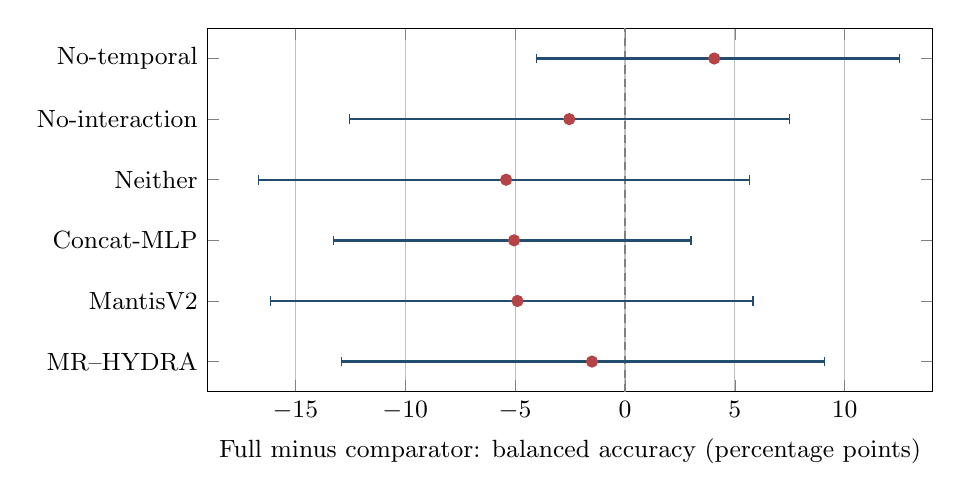
\begin{tikzpicture}\begin{axis}[width=.89\linewidth,height=6.2cm,xmin=-19,xmax=14,ymin=.5,ymax=6.5,ytick={1,2,3,4,5,6},yticklabels={MR--HYDRA,MantisV2,Concat-MLP,Neither,No-interaction,No-temporal},xlabel={Full minus comparator: balanced accuracy (percentage points)},xmajorgrids,tick label style={font=\small},label style={font=\small}]
\draw[densely dashed,gray] (axis cs:0,.5)--(axis cs:0,6.5);
\draw[navy,line width=.9pt] (axis cs:-4.0146221532091095,6)--(axis cs:12.474120082815734,6);
\draw[navy] (axis cs:-4.0146221532091095,5.92)--(axis cs:-4.0146221532091095,6.08);
\draw[navy] (axis cs:12.474120082815734,5.92)--(axis cs:12.474120082815734,6.08);
\addplot[only marks,mark=*,redplot,mark size=2pt] coordinates {(4.063146997929606,6)};
\draw[navy,line width=.9pt] (axis cs:-12.55175983436853,5)--(axis cs:7.479296066252589,5);
\draw[navy] (axis cs:-12.55175983436853,4.92)--(axis cs:-12.55175983436853,5.08);
\draw[navy] (axis cs:7.479296066252589,4.92)--(axis cs:7.479296066252589,5.08);
\addplot[only marks,mark=*,redplot,mark size=2pt] coordinates {(-2.536231884057971,5)};
\draw[navy,line width=.9pt] (axis cs:-16.666666666666664,4)--(axis cs:5.667701863354037,4);
\draw[navy] (axis cs:-16.666666666666664,3.92)--(axis cs:-16.666666666666664,4.08);
\draw[navy] (axis cs:5.667701863354037,3.92)--(axis cs:5.667701863354037,4.08);
\addplot[only marks,mark=*,redplot,mark size=2pt] coordinates {(-5.408902691511387,4)};
\draw[navy,line width=.9pt] (axis cs:-13.250517598343686,3)--(axis cs:3.002070393374741,3);
\draw[navy] (axis cs:-13.250517598343686,2.92)--(axis cs:-13.250517598343686,3.08);
\draw[navy] (axis cs:3.002070393374741,2.92)--(axis cs:3.002070393374741,3.08);
\addplot[only marks,mark=*,redplot,mark size=2pt] coordinates {(-5.046583850931677,3)};
\draw[navy,line width=.9pt] (axis cs:-16.1231884057971,2)--(axis cs:5.823628364389229,2);
\draw[navy] (axis cs:-16.1231884057971,1.92)--(axis cs:-16.1231884057971,2.08);
\draw[navy] (axis cs:5.823628364389229,1.92)--(axis cs:5.823628364389229,2.08);
\addplot[only marks,mark=*,redplot,mark size=2pt] coordinates {(-4.891304347826087,2)};
\draw[navy,line width=.9pt] (axis cs:-12.914725672877847,1)--(axis cs:9.061853002070372,1);
\draw[navy] (axis cs:-12.914725672877847,0.92)--(axis cs:-12.914725672877847,1.08);
\draw[navy] (axis cs:9.061853002070372,0.92)--(axis cs:9.061853002070372,1.08);
\addplot[only marks,mark=*,redplot,mark size=2pt] coordinates {(-1.5010351966873712,1)};
\end{axis}\end{tikzpicture}
\caption{대응 BA 차이의 조건부 구간. 0보다 오른쪽이면 Full이 높다.
모든 구간이 0을 포함한다. 이 사실은 동등성을 증명하거나
재학습을 포함하는 모든 불확실성 아래 차이가 없음을 증명하지 않는다.}
\end{figure}
이번 실행에서 Full의 성능 향상을 뒷받침하는 근거는 확보되지 않았다.
반면 Neither의 BA가 가장 높다는 순위도 이 작은 코호트의 기술적 관측이며,
보편적인 최적 모델 선택 결론은 아니다.

\section{학습 기록, 계산 비용과 최종 모델}
\subsection{학습 손실의 관찰}
\begin{figure}[H]\centering
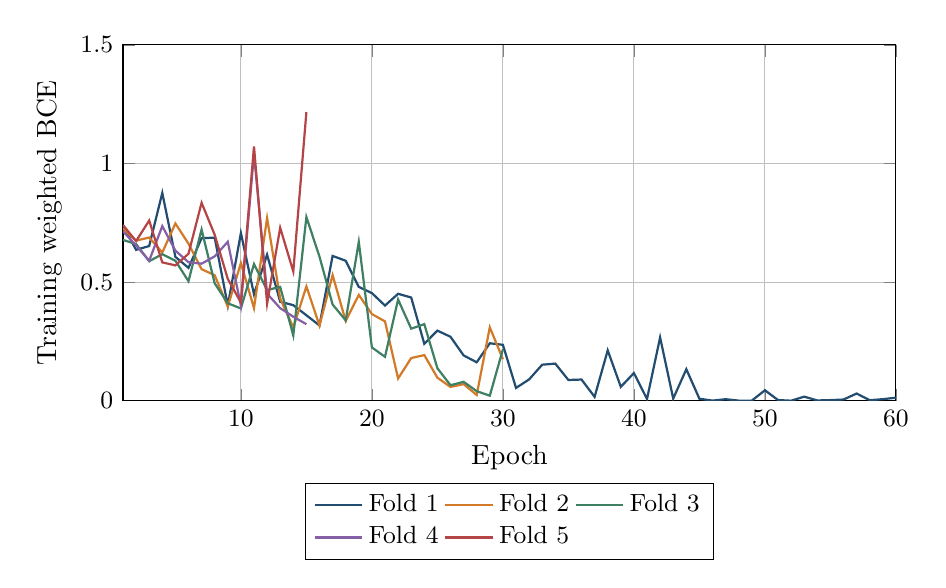
\begin{tikzpicture}\begin{axis}[width=.94\linewidth,height=6.1cm,xlabel={Epoch},ylabel={Training weighted BCE},xmin=1,xmax=60,ymin=0,ymax=1.5,grid=major,legend columns=3,legend style={at={(.5,-.23)},anchor=north,font=\small},tick label style={font=\small}]
\addplot[thick,navy,no marks] coordinates {(1,0.73836488) (2,0.63611281) (3,0.65214411) (4,0.87594207) (5,0.60640247) (6,0.56012931) (7,0.68497788) (8,0.68763245) (9,0.40085714) (10,0.70705818) (11,0.44852899) (12,0.61560173) (13,0.41727288) (14,0.40273912) (15,0.36024843) (16,0.31719659) (17,0.61044925) (18,0.59002855) (19,0.47982134) (20,0.45374741) (21,0.40111687) (22,0.45079351) (23,0.43505969) (24,0.23979177) (25,0.29554037) (26,0.26954119) (27,0.19093902) (28,0.16197096) (29,0.24215043) (30,0.23562073) (31,0.053825698) (32,0.08972368) (33,0.15181277) (34,0.15631901) (35,0.087372684) (36,0.089193678) (37,0.016310274) (38,0.21220739) (39,0.05845961) (40,0.11649517) (41,0.0073452219) (42,0.266892) (43,0.0089274898) (44,0.13269933) (45,0.0083250606) (46,0.00035916196) (47,0.0062788652) (48,0.00033782283) (49,0.00030428137) (50,0.044057489) (51,0.002684249) (52,7.2001583e-05) (53,0.017024695) (54,0.0010573947) (55,0.0025248178) (56,0.0048723195) (57,0.030186515) (58,0.0020730123) (59,0.0064590518) (60,0.012683933)};
\addlegendentry{Fold 1}
\addplot[thick,orangeplot,no marks] coordinates {(1,0.72628399) (2,0.67473131) (3,0.68811843) (4,0.62486109) (5,0.74710187) (6,0.66202718) (7,0.55447116) (8,0.52902538) (9,0.39673318) (10,0.58051536) (11,0.39036549) (12,0.76976495) (13,0.43074342) (14,0.30897822) (15,0.48172759) (16,0.31670787) (17,0.52960008) (18,0.33638089) (19,0.44602642) (20,0.36520865) (21,0.33450039) (22,0.093649201) (23,0.17973283) (24,0.19229399) (25,0.096937512) (26,0.058016411) (27,0.070039593) (28,0.02417165) (29,0.30950805) (30,0.17503492)};
\addlegendentry{Fold 2}
\addplot[thick,greenplot,no marks] coordinates {(1,0.67807618) (2,0.66012387) (3,0.58813722) (4,0.61780516) (5,0.59015998) (6,0.50378329) (7,0.7218076) (8,0.49496369) (9,0.41065133) (10,0.3890543) (11,0.57595877) (12,0.46664542) (13,0.47977028) (14,0.27490431) (15,0.77428146) (16,0.6074054) (17,0.40561066) (18,0.33895307) (19,0.66936377) (20,0.22457486) (21,0.18510147) (22,0.4266618) (23,0.30365761) (24,0.32281155) (25,0.13683293) (26,0.065304294) (27,0.079573137) (28,0.040204573) (29,0.021010258) (30,0.21661135)};
\addlegendentry{Fold 3}
\addplot[thick,purpleplot,no marks] coordinates {(1,0.71450837) (2,0.65420708) (3,0.59031316) (4,0.73616119) (5,0.6328561) (6,0.5838963) (7,0.57773152) (8,0.6085379) (9,0.67010846) (10,0.40086838) (11,1.0417031) (12,0.45143486) (13,0.39012301) (14,0.35415595) (15,0.32256165)};
\addlegendentry{Fold 4}
\addplot[thick,redplot,no marks] coordinates {(1,0.74052449) (2,0.67288906) (3,0.75962032) (4,0.5831181) (5,0.57050442) (6,0.61957895) (7,0.83436143) (8,0.69973267) (9,0.51334984) (10,0.41430185) (11,1.0719964) (12,0.4087678) (13,0.72914205) (14,0.54459975) (15,1.2171471)};
\addlegendentry{Fold 5}
\end{axis}\end{tikzpicture}
\caption{Full의 외부 학습 집합 재학습 중 기록된 가중 BCE.
각 epoch 값은 dropout이 켜진 미니배치 갱신 중 손실을 배치 인원으로 가중 평균한
값이다. 같은 epoch 종료 시점 모델을 전체 학습 자료에 평가 모드로 적용한 손실이 아니다.
곡선 길이는 내부에서 선택한 60, 30, 30, 15, 15 epoch를 따른다.}
\label{fig:training}
\end{figure}
Full fold 1의 마지막 학습 손실은 약 0.0127이지만 외부 성능 개선으로 이어지지
않았다. fold 5의 마지막 기록은 약 1.2171로 첫 기록 약 0.7405보다 높다.
매우 낮은 학습 손실과 일부 비단조 기록은 추가 진단의 근거가 될 수 있다.
다만 위 기록에는 배치 구성, 드문 ET 사례의 가중치, dropout과 갱신 중 모수 변화가
함께 반영된다. 검증 손실 곡선을 저장하지 않았으므로 이 그림만으로 과적합의
발생 시점이나 최적화 불안정성의 원인을 확정하지 않는다.

\subsection{모수 수와 소요 시간}
\begin{table}[H]\centering\small
\caption{신경망의 학습 가능한 모수 수. 기본 Full은 24,425개다.}
\begin{tabular}{@{}lr@{}}\toprule 모델 & 학습 가능한 모수\\\midrule
Full & 24,425 \\
No-temporal & 15,881 \\
No-interaction & 22,313 \\
Neither & 13,769 \\
Concat-MLP & 30,826 \\
\bottomrule\end{tabular}
\end{table}
실행 장치는 신경망과 MantisV2 특징 추출에 Apple MPS, HYDRAㆍMultiROCKETㆍ
ridge 및 특징 scaler에 CPU를 사용하였다. CPU thread 설정은 4다.
\begin{table}[H]\centering\small
\caption{저장된 외부 fold 경과 시간 합계(초). 내부 탐색과 외부 재학습ㆍ예측을
포함하며, 순수 학습/추론 벤치마크가 아니다.}
\begin{tabular}{@{}lrl@{}}\toprule 모델 & 외부 5개 fold 시간 합계 & 실행 경로\\\midrule
Full & 585.18 & MPS + CPU \\
No-temporal & 283.50 & MPS + CPU \\
No-interaction & 388.50 & MPS + CPU \\
Neither & 287.76 & MPS + CPU \\
Concat-MLP & 578.90 & MPS + CPU \\
MantisV2 & 3.28 & CPU (고정 특징) \\
MR--HYDRA & 306.62 & CPU \\
\bottomrule\end{tabular}\label{tab:runtime}
\end{table}
MantisV2의 표 시간에는 공통 고정 특징 추출 11.76초가 제외되어 있다.
전체 실행은 한국 시각 2026-11-08 16:17:20부터 2026-11-08 17:00:32까지이며,
기록된 총 경과 시간은 2592.25초(약 43분 12초)다.
전체에는 데이터 읽기, 특징 추출, 저장과 별도의 최종 모델 선택ㆍ적합도 포함된다.
환경 준비와 다운로드 시간의 공정한 비교나 장치 간 가속도 비교를 수행하지 않았다.

\subsection{전체 참가자로 적합한 최종 모델}
외부 평가가 끝난 뒤 전체 304명에서 별도의 내부 3-fold 탐색을 수행하여
Full의 weight decay 0.01, 30 epoch, 임계값 0을 선택하고 새로 적합하였다.
내부 평균 BA 59.55\%는 최종 설정 선택에 사용한 값으로, 새로운 외부 성능이 아니다.
\code{final_model.pt}에는 24,425개 학습 모수와 설정, 표준화 통계, 임계값,
학습 참가자 ID, 패키지 버전과 소스 해시가 저장되어 있다.
보고서 작성 시 저장 tensor의 유한성과 메타데이터 일치만 확인했으며,
이 모델을 참가자에게 다시 적용하지 않았다.

\section{해석의 한계와 후속 실험}
\subsection{이번 결과가 지지하는 범위}
이번 특정 CNN--Transformer--쌍선형 결합은 고정 임계값의 BA에서
동일 입력의 두 기준선을 개선하지 못했다. ET 민감도도 충분히 높지 않았다.
따라서 임상적 개선이나 새로운 최고 성능을 주장할 수 없다.
동시에 제한된 은닉 차원, 단일 초기화와 좁은 후보 목록의 한 결과로
시간 표현 또는 과제 간 관계 정보 자체가 쓸모없다고 결론내릴 수 없다.

ET는 28명뿐이다. ET 한 명의 정오분류가 바뀌면 민감도는 약 3.57\%p,
PD 판정이 같을 때 BA는 약 1.79\%p 변한다. 외부 fold의 ET는 5--6명,
내부 실제 학습 ET는 14--16명이다. 윈도 수 증가는 독립 참가자 수 증가가 아니다.
단일 기관의 기존 코호트를 여러 차례 분석했으며 외부ㆍ전향 검증은 없다.

또한 PADS의 모든 PD 사례가 반드시 떨림 우세형인 것은 아니다.
PD/ET 진단 분류 성능을 떨림 표현형만의 구별력과 동일시하지 않는다.
정답은 공개 임상 진단이며 독립 재진단을 하지 않았다.
공식 전처리의 중력 추정, 구간 선택, 비균일 원자료 시간 간격과 신호 품질이
잠재 특징에 미친 영향을 이번 실험에서 분해하지 않았다.

\subsection{이미 관측한 외부 성능을 재사용하지 않는 개선 방향}
\begin{enumerate}
 \item \textbf{단순 대조군을 유지한다.} Neither와 고정 표현 기준선을 포함하여,
 명시적 진폭ㆍ주파수 변화 통계가 필요한지와 모델 복잡도의 효과를 구분한다.
 지연된 과제 효과를 생리적으로 주장하려면 별도의 해석 검증이 필요하다.
 \item \textbf{원자료 시간축을 검증한다.} 실제 타임스탬프 기반 재표본화와 긴 간격의
 처리 규칙을 미리 정하고, 동일 품질 처리와 동일 코호트를 모든 방법에 적용한다.
 신호 품질 제외로 ET가 줄어드는 선택 편향도 함께 보고한다.
 \item \textbf{정규화ㆍ학습 안정성을 내부에서만 조정한다.} 두 기준선의 모든 외부
 fold가 ridge alpha 1000을 선택했으므로 탐색 상단이 충분한지 검증할 여지가 있다.
 더 넓은 alpha, 신경망 학습률과 학습 규칙은 새로운 탐색으로 명시해야 한다.
 \item \textbf{임계값 절차를 별도 검증한다.} 높은 AUROC와 낮은 ET 민감도가 공존하는
 기준선에서 내부 검증 기반 임계값 선택 또는 임상적으로 정한 특이도 조건을
 검토할 수 있다. 현재 외부 정답으로 가장 좋은 임계값을 고른 값을 새 성능으로 쓰지 않는다.
 \item \textbf{변동성과 외부 일반화를 확보한다.} 초기화ㆍ분할 반복은 안정성 점검에
 쓰되 참가자 수를 늘렸다고 간주하지 않는다. 새로운 ET 참가자와 외부 기관 코호트가
 확증적 검증에 필요하다.
\end{enumerate}

\section{결론}
동일한 세 조건ㆍ60채널 입력과 참가자 단위 중첩 교차검증에서,
전체 제안 모델의 BA는 56.16\%, ET 민감도는 25.00\%, PD 특이도는 87.32\%였다.
Neither는 BA 61.57\%, MantisV2는 61.05\%였고,
MR--HYDRA는 pooled AUROC 0.8612로 가장 높은 순위 지표를 보였다.
구성요소 제거 결과는 두 모듈의 결합이 성능을 개선한다는 가설을 지지하지 않았다.
후속 연구는 단순한 대조군을 유지하면서 시간축 품질, 정규화ㆍ최적화,
내부 임계값 선택과 외부 ET 표본을 검증하는 방향으로 진행하는 것이 타당하다.

\clearpage\appendix
\section{모든 외부 fold의 선택 설정과 평가 결과}
\small
신경망의 설정 열은 ``epoch / weight decay'', 기준선은 ridge alpha다.
내부 BA는 설정 선택용 3개 fold 평균, 외부 BA는 해당 외부 평가 참가자의 값이다.
각 fold의 평가 인원은 표~\ref{tab:splits}를 따른다. 모든 임계값은 0이다.
\begin{longtable}{@{}lclrrrr@{}}
\caption{35개 외부 fold의 설정과 결과. BA는 \%, AUROC는 0--1이다.}\label{tab:allfolds}\\
\toprule 모델 & fold & 설정 & 내부 BA & 외부 BA & ET 정분류 & AUROC\\\midrule\endfirsthead
\toprule 모델 & fold & 설정 & 내부 BA & 외부 BA & ET 정분류 & AUROC\\\midrule\endhead
\midrule\multicolumn{7}{r}{다음 페이지에 계속}\\\endfoot
\bottomrule\endlastfoot
Full & 1 & 60 / 0.01 & 65.26 & 56.43 & 1/5 & 0.7250 \\
Full & 2 & 30 / 0.01 & 62.38 & 52.88 & 1/6 & 0.7152 \\
Full & 3 & 30 / 0.01 & 62.64 & 50.15 & 1/6 & 0.4485 \\
Full & 4 & 15 / 0.01 & 58.38 & 65.00 & 3/6 & 0.7636 \\
Full & 5 & 15 / 0.001 & 60.76 & 55.45 & 1/5 & 0.6727 \\
No-temporal & 1 & 30 / 0.001 & 60.14 & 48.21 & 0/5 & 0.7429 \\
No-temporal & 2 & 15 / 0.001 & 60.16 & 63.03 & 2/6 & 0.7879 \\
No-temporal & 3 & 15 / 0.01 & 62.34 & 44.55 & 0/6 & 0.6152 \\
No-temporal & 4 & 15 / 0.01 & 58.10 & 54.70 & 1/6 & 0.8091 \\
No-temporal & 5 & 15 / 0.01 & 62.02 & 48.18 & 0/5 & 0.6655 \\
No-interaction & 1 & 30 / 0.001 & 58.70 & 58.21 & 1/5 & 0.7179 \\
No-interaction & 2 & 15 / 0.01 & 58.65 & 62.12 & 2/6 & 0.8091 \\
No-interaction & 3 & 60 / 0.001 & 66.83 & 60.30 & 2/6 & 0.4636 \\
No-interaction & 4 & 15 / 0.01 & 58.02 & 63.03 & 2/6 & 0.8091 \\
No-interaction & 5 & 15 / 0.01 & 62.55 & 47.27 & 0/5 & 0.6509 \\
Neither & 1 & 15 / 0.001 & 56.82 & 66.43 & 2/5 & 0.8071 \\
Neither & 2 & 15 / 0.01 & 57.17 & 73.18 & 3/6 & 0.7818 \\
Neither & 3 & 15 / 0.01 & 63.06 & 53.79 & 1/6 & 0.6485 \\
Neither & 4 & 15 / 0.01 & 57.37 & 64.85 & 2/6 & 0.8606 \\
Neither & 5 & 15 / 0.01 & 63.42 & 48.18 & 0/5 & 0.6545 \\
Concat-MLP & 1 & 15 / 0.01 & 61.69 & 59.11 & 1/5 & 0.8107 \\
Concat-MLP & 2 & 60 / 0.001 & 57.17 & 47.27 & 0/6 & 0.6394 \\
Concat-MLP & 3 & 15 / 0.01 & 63.06 & 60.30 & 2/6 & 0.6242 \\
Concat-MLP & 4 & 15 / 0.01 & 56.37 & 81.52 & 4/6 & 0.8515 \\
Concat-MLP & 5 & 15 / 0.01 & 58.22 & 56.36 & 1/5 & 0.6873 \\
MantisV2 & 1 & $\alpha=1000$ & 53.32 & 59.11 & 1/5 & 0.8857 \\
MantisV2 & 2 & $\alpha=1000$ & 58.10 & 74.09 & 3/6 & 0.7212 \\
MantisV2 & 3 & $\alpha=1000$ & 64.94 & 48.18 & 0/6 & 0.6818 \\
MantisV2 & 4 & $\alpha=1000$ & 60.33 & 73.18 & 3/6 & 0.9424 \\
MantisV2 & 5 & $\alpha=1000$ & 57.27 & 48.18 & 0/5 & 0.8218 \\
MR--HYDRA & 1 & $\alpha=1000$ & 57.27 & 49.11 & 0/5 & 0.8464 \\
MR--HYDRA & 2 & $\alpha=1000$ & 55.94 & 74.09 & 3/6 & 0.8515 \\
MR--HYDRA & 3 & $\alpha=1000$ & 58.09 & 56.52 & 1/6 & 0.8576 \\
MR--HYDRA & 4 & $\alpha=1000$ & 53.26 & 57.42 & 1/6 & 0.9091 \\
MR--HYDRA & 5 & $\alpha=1000$ & 55.19 & 48.18 & 0/5 & 0.8982 \\
\end{longtable}
\normalsize

\section{보조 지표와 과거 결과의 구분}
\begin{table}[H]\centering\small
\caption{동일 60채널 실험의 보조 지표. 정확도와 ET precision은 \%,
F1은 $[0,1]$, MCC는 $[-1,1]$ 척도다.}
\begin{tabular}{@{}lrrrrr@{}}\toprule
 모델 & 정확도 & ET precision & ET F1 & macro-F1 & MCC\\\midrule
Full & 81.58 & 16.67 & 0.2000 & 0.5480 & 0.1032 \\
No-temporal & 85.86 & 14.29 & 0.1224 & 0.5228 & 0.0478 \\
No-interaction & 86.18 & 25.00 & 0.2500 & 0.5870 & 0.1739 \\
Neither & 88.49 & 34.78 & 0.3137 & 0.6254 & 0.2530 \\
Concat-MLP & 87.83 & 32.00 & 0.3019 & 0.6176 & 0.2359 \\
MantisV2 & 90.46 & 46.67 & 0.3256 & 0.6371 & 0.2951 \\
MR--HYDRA & 90.13 & 41.67 & 0.2500 & 0.5986 & 0.2275 \\
\bottomrule\end{tabular}
\end{table}

\begin{table}[H]\centering\small
\caption{과거 132채널과 이번 60채널의 기준선 결과. 입력 범위가 달라 직접적인
동일 입력 모델 비교로 취급하지 않는다. BA는 \%, AUROC는 pooled 값이다.}
\begin{tabular}{@{}lrrrr@{}}\toprule
 모델 & 입력 채널 & BA & ET 정분류 & AUROC\\\midrule
MantisV2 & 132 & 70.89 & 12/28 & 0.8876 \\
MR--HYDRA & 132 & 67.13 & 10/28 & 0.9000 \\
MantisV2 & 60 & 61.05 & 7/28 & 0.8056 \\
MR--HYDRA & 60 & 57.66 & 5/28 & 0.8612 \\
\bottomrule\end{tabular}\label{tab:historical}
\end{table}
과거 두 실행은 이번과 같은 참가자ㆍ분할을 쓰지만 더 많은 과제 구간을 포함한다.
이번 기준선의 성능이 과거보다 낮은 사실은 관측되지만, 과제 제거의 순수한 인과
효과로 볼 수는 없다. 입력 차원에 따른 무작위 특징 구성과 ridge 선택 등이 함께
달라진다. 132채널 기준선과 60채널 Full을 직접 비교해 구조 차이만의 효과로
주장하지 않는다. 본문의 주 비교는 모두 60채널 실험이다.

\section{감사, 재현성과 문서 생성}
\subsection{저장 결과의 독립 재계산}
보고서 작성은 완료된 결과 파일을 읽는 분석이며 모델을 학습하거나 예측하지 않았다.
참가자 IDㆍ라벨ㆍ내부/외부 분리와 예측 커버리지를 검사하고,
일곱 방법의 pooled 지표와 35개 외부 fold 지표를 scikit-learn으로 다시 계산하였다.
선택된 내부 OOF 예측으로 내부 평균 BA를 재계산하고, 후보 최대값 및 동점 규칙과
일치함을 확인하였다. 여섯 대응 BA 차이와 조건부 bootstrap 구간도 다시 계산하였다.

추가로 실행 manifest가 기록한 원 데이터ㆍ정의 파일 611개의 SHA-256,
실행 시점 소스 23개의 보관본 SHA-256을 검증하였다.
Mantis 고정 특징 캐시의 모양 $(304,30720)$과 해시,
최종 모델의 학습 IDㆍ유한 tensorㆍ소스 해시도 일치하였다.
모든 비교 수치 차이는 $10^{-12}$ 이내였다.
이는 저장 자료와 계산ㆍ소스의 일관성 감사이며, 학습을 다시 실행한 재현 실험이나
모든 학습 연산을 관찰한 실행 추적 증명은 아니다.

\begin{table}[H]\centering\small
\caption{완료 실행에 기록된 주요 패키지 버전.}
\begin{tabular}{@{}lr@{}}\toprule 패키지 & 버전\\\midrule
\code{numpy} & 2.3.5 \\
\code{scipy} & 1.17.1 \\
\code{scikit-learn} & 1.9.1 \\
\code{torch} & 2.14.1 \\
\code{aeon} & 1.6.0 \\
\code{mantis-tsfm} & 1.1.0 \\
\code{joblib} & 1.6.0 \\
\code{threadpoolctl} & 3.7.0 \\
\code{safetensors} & 0.8.0 \\
\bottomrule\end{tabular}
\end{table}

\subsection{재현 파일과 보고서 빌드}
실행 식별자는 \code{20261108T071720522119Z}이며 원본 결과는 프로젝트의
\path{artifacts/pads_temporal_cross_task/20261108T071720522119Z/}에 있다.
주요 근거 파일은 다음과 같다.
\begin{itemize}
 \item \code{manifest.json}, \code{splits.json}, \code{cohort.csv}: 설정, 소스ㆍ자료 해시와 분할.
 \item 모델별 \code{oof_predictions.csv}, fold별 \code{test_predictions.csv}: 외부 평가의 직접 근거.
 \item fold별 \code{inner_search.csv}, \code{inner_oof_predictions.csv}, \code{selected.json}: 선택 근거.
 \item \code{paired_comparisons.json}: 대응 BA 차이와 조건부 bootstrap 구간.
 \item \code{evaluated_sources.zip}, \code{final_model.pt}: 실행 소스와 최종 적합 객체.
\end{itemize}
보고서 폴더의 \code{build_report.py}는 위 파일을 감사하고 수치ㆍ좌표를 삽입한
\code{report.tex}, \code{verification.json}, \code{metrics.csv}를 생성한다.
생성된 \code{report.tex}에는 표와 벡터 그림 좌표가 모두 들어 있어
원본 결과 파일이나 외부 이미지 없이 XeLaTeX로 컴파일할 수 있다.
\begin{lstlisting}
latexmk -xelatex -interaction=nonstopmode -halt-on-error report.tex
\end{lstlisting}
한국어 처리는 ko.TeX, 글꼴은 TeX Live의 UnBatang을 사용한다.
모든 그래프는 PGFPlots/TikZ 벡터 그림이며, 숫자와 좌표는 저장된 예측과 지표에서 생성했다.
데이터 이용 및 재배포는 PADS의 CC BY-NC-SA 4.0 조건과 공식 인용 지침을 따른다\cite{pads,physionet}.

\clearpage
\begin{thebibliography}{9}
\bibitem{pads} J. Varghese, A. Brenner, L. Plagwitz, C. van Alen, M. Fujarski, and T. Warnecke.
\emph{PADS -- Parkinsons Disease Smartwatch dataset}, version 1.0.0, PhysioNet, 2024.
\url{https://doi.org/10.13026/m0w9-zx22}.
\bibitem{padsstudy} J. Varghese et al.
Machine Learning in the Parkinson's disease smartwatch (PADS) dataset.
\emph{npj Parkinson's Disease}, 10:9, 2024.
\url{https://doi.org/10.1038/s41531-023-00625-7}.
\bibitem{physionet} A. L. Goldberger et al.
PhysioBank, PhysioToolkit, and PhysioNet: components of a new research resource for complex physiologic signals.
\emph{Circulation}, 101(23):e215--e220, 2000.
\url{https://doi.org/10.1161/01.CIR.101.23.e215}.
\bibitem{multirocket} C. W. Tan, A. Dempster, C. Bergmeir, and G. I. Webb.
MultiRocket: multiple pooling operators and transformations for fast and effective time series classification.
\emph{Data Mining and Knowledge Discovery}, 36:1623--1646, 2022.
\url{https://doi.org/10.1007/s10618-022-00844-1}.
\bibitem{hydra} A. Dempster, D. F. Schmidt, and G. I. Webb.
Hydra: competing convolutional kernels for fast and accurate time series classification.
\emph{Data Mining and Knowledge Discovery}, 37:1779--1805, 2023.
\url{https://doi.org/10.1007/s10618-023-00939-3}.
\bibitem{mantis} V. Feofanov, S. Wen, J. Zhang, L. Pan, and I. Redko.
MantisV2: Closing the Zero-Shot Gap in Time Series Classification with Synthetic Data and Test-Time Strategies.
arXiv:2602.17868, 2026. \url{https://arxiv.org/abs/2602.17868}.
\bibitem{tsi} L. di Biase et al.
Tremor stability index: a new tool for differential diagnosis in tremor syndromes.
\emph{Brain}, 140(7):1977--1986, 2017.
\url{https://doi.org/10.1093/brain/awx104}.
\bibitem{mfca} L. Tang et al.
A multimodal fusion network based on a cross-attention mechanism for the classification of Parkinsonian tremor and essential tremor.
\emph{Scientific Reports}, 14:28050, 2024.
\url{https://doi.org/10.1038/s41598-024-79111-w}.
\bibitem{bilateral} M. Zannat.
Label-Efficient Bilateral Attention for Parkinson's Disease Screening from Wrist-Worn IMU Signals.
arXiv:2604.18372v2, 2026. \url{https://arxiv.org/abs/2604.18372v2}.
\end{thebibliography}
\end{document}
